%\documentclass{article}
%\usepackage[T1]{fontenc}
%\usepackage[utf8]{inputenc}
%\usepackage{amsmath}
%\usepackage{amssymb}
%\usepackage{hyperref}
%\usepackage{parskip} %skip the indent of a new paragraph.
%\usepackage{float}
%\usepackage{graphicx}
%\usepackage{siunitx}
%\usepackage{listings}
%\usepackage{placeins}


\documentclass[pdftex,10pt,b5paper,twoside]{book}
\usepackage[lmargin=25mm,rmargin=25mm,tmargin=27mm,bmargin=30mm]{geometry}

\usepackage{setspace}
\usepackage{graphicx}
\usepackage{amssymb}
\usepackage{mathrsfs}
\usepackage{amsthm}
\usepackage{amsmath}

% for multiline equations autosplit
\usepackage{breqn}

%\usepackage[norsk]{babel}  % norske navn rundt omkring
%\usepackage[T1]{fontenc}   % norsk tegnsett (æøå)
%\usepackage[latin1]{inputenc} 

% Create argmin and argmax functions
\DeclareMathOperator*{\argmin}{argmin}   % Jan Hlavacek
\DeclareMathOperator*{\argmax}{argmax}   % Jan Hlavacek

\usepackage{color}
\usepackage[Lenny]{fncychap}
\usepackage[pdftex,bookmarks=true]{hyperref}
\usepackage[pdftex]{hyperref}
\hypersetup{
    colorlinks,%
    citecolor=black,%
    filecolor=black,%
    linkcolor=black,%
    urlcolor=black
}
\usepackage[font=small,labelfont=bf]{caption}
\usepackage{fancyhdr}
\usepackage{times}

% SI units and signs
\usepackage{siunitx}

% Write "Figures" instead of "List of Figures"
\renewcommand{\listfigurename}{Figures}

% Increase size of todos
%\setlength{\marginparwidth}{4cm}


%% Temporarily increase size of paper to add room for todos. REMEMBER TO REMOVE THIS FFS!
%\paperwidth=\dimexpr \paperwidth + 6cm\relax
%\oddsidemargin=\dimexpr\oddsidemargin + 3cm\relax
%\evensidemargin=\dimexpr\evensidemargin + 3cm\relax
%\marginparwidth=\dimexpr \marginparwidth + 3cm\relax



%\usepackage[intoc]{nomencl}
%\renewcommand{\nomname}{List of Abbreviations}
%\makenomenclature
\usepackage{natbib}
\usepackage{float}
%\floatstyle{boxed} 
\restylefloat{figure}

% ShareLaTeX does not support glossaries now. Sorry...
%\usepackage[number=none]{glossary}
%\makeglossary
%\newglossarytype[abr]{abbr}{abt}{abl}
%\newglossarytype[alg]{acronyms}{acr}{acn}
%\newcommand{\abbrname}{Abbreviations} 
%\newcommand{\shortabbrname}{Abbreviations}
%%\makeabbr
\newcommand{\HRule}{\rule{\linewidth}{0.5mm}}

\renewcommand*\contentsname{Table of Contents}

\pagestyle{fancy}
\fancyhf{}
\renewcommand{\chaptermark}[1]{\markboth{\chaptername\ \thechapter.\ #1}{}}
\renewcommand{\sectionmark}[1]{\markright{\thesection\ #1}}
\renewcommand{\headrulewidth}{0.1ex}
\renewcommand{\footrulewidth}{0.1ex}
\fancypagestyle{plain}{\fancyhf{}\fancyfoot[LE,RO]{\thepage}\renewcommand{\headrulewidth}{0ex}}


\usepackage{cleveref}
\usepackage{todonotes}

\title{State estimation, mapping and localization of autonomous race car for Revolve NTNU}
\author{Adrian Bogen Skibelid}
\date{2019}

\begin{document}

%\begin{titlepage}
%    \maketitle
%    \rule{\linewidth}{0.5mm}
%    \begin{figure}
%    \centering
%    
\includegraphics[width=0.5\textwidth]{0_Images/logontnu.pdf}
%    \end{figure}
%    %\thispagestyle{empty}
%\end{titlepage}
\begin{titlepage} % Suppresses displaying the page number on the title page and the subsequent page counts as page 1
	\newcommand{\HRule}{\rule{\linewidth}{0.5mm}} % Defines a new command for horizontal lines, change thickness here
	
	\center % Centre everything on the page
	
	%------------------------------------------------
	%	Headings
	%------------------------------------------------
	
	%\textsc{\LARGE Institution Name}\\[1.5cm] % Main heading such as the name of your university/college
	
	%\textsc{\Large Major Heading}\\[0.5cm] % Major heading such as course name
	
	%\textsc{\large Minor Heading}\\[0.5cm] % Minor heading such as course title
	
	%------------------------------------------------
	%	Title
	%------------------------------------------------
	
	\HRule\\[0.4cm]
	
	{\huge\bfseries 
	{\setstretch{1.0}
	State estimation, mapping and localization of autonomous race car for Revolve NTNU}\\[0.4cm] % Title of your document
	}
	
	\HRule\\[1.5cm]
	
	%------------------------------------------------
	%	Author(s)
	%------------------------------------------------
	
	\begin{minipage}{0.4\textwidth}
		\begin{flushleft}
			\large
			\textit{Author}\\
			\textsc{Adrian B. Skibelid} % Your name
		\end{flushleft}
	\end{minipage}
	~
	\begin{minipage}{0.4\textwidth}
		\begin{flushright}
			\large
			\textit{Supervisor}\\
			\textsc{Trym V. Haavardsholm} % Supervisor's name
		\end{flushright}
	\end{minipage}
	
	% If you don't want a supervisor, uncomment the two lines below and comment the code above
	%{\large\textit{Author}}\\
	%John \textsc{Smith} % Your name
	
	%------------------------------------------------
	%	Date
	%------------------------------------------------
	
	\vfill\vfill\vfill % Position the date 3/4 down the remaining page
	
	{\large\today} % Date, change the \today to a set date if you want to be precise
	
	%------------------------------------------------
	%	Logo
	%------------------------------------------------
	
	\vfill\vfill
	
\includegraphics[width=0.6\textwidth]{0_Images/logontnu.pdf}\\[1cm] % Include a department/university logo - this will require the graphicx package
	 
	%----------------------------------------------------------------------------------------
	
	\vfill % Push the date up 1/4 of the remaining page
	
\end{titlepage}
\let\cleardoublepage\clearpage
%----------------------------------------------------------------------------------------


%\section*{Table of contents} 
\tableofcontents
\listoffigures
\thispagestyle{empty} %Avoid page numbering on the table of contents
\newpage    

\setcounter{page}{1}
\let\cleardoublepage\clearpage
\chapter{Abstract}
I don't know what to write here yet, need to check out other abstracts to get a proper feel for how an abstract should be.
%\let\cleardoublepage\clearpage
\chapter{Introduction}
\section{Formula student driverless}

This project thesis is done as part of Revolve NTNU, a team competing in various competitions around Europe in what is known as Formula Student. Formula Student is often referred to as the worlds largest engineering competition, while in reality it consists of several competitions spread around the globe, one of the msot influential of which is Formula Student Germany (FSG). FSG 2018 had over 300 students in 66 teams from 8 different countries. \\

Each competition follows more or less the same recipe; build a car that gets through, the very strict, scrutineering, where every aspect of the car must follow an intense safety and quality protocol demanded by the competition. If the car passes it competes in one of three classes: combustion, electric or driverless. \\ 

This implies both static and dynamic events, where the static are focused on cost, documentation of the engineering process, and so on. The dynamic events for the combustion and electric class encompasses showing how energy efficient the car is, how well it accelerates, corners and so on. \\ 

The driverless class is a rather new one, only being introduced at FSG in 2017. Revolve NTNU had it's first driverless team in 2018. Each driverless car is tested in four dynamic events: Acceleration, Skidpad, autocross and trackdrive. Each of the events are to be done without a driver in the car and without signals being sent to the car from the team in any way. In all events the goal is to drive as fast as possible without knocking any delimiters, which are blue cones on the left side and yellow cones on the right. Knocking a delimiter gives a time penalty.\\

The acceleration event is just a 75 meter straight path, very much akin to a drag race. Skidpad has the car driving in a figure eight pattern, taking two loops on each circle, only being timed on the second run of each circle. Autocross is one round of an unknown track, where it isn't allowed to do any mapping before starting the event. Trackdrive is the same as autocross, only now driving 10 rounds. \\

Each event therefore requires somewhat different approaches. What is however constant is the need for good state estimation, detection, localization and mapping, so the car can drive fast without hitting any delimiters.
\section{Problem formulation}
Estimate local changes in the states using sensor data; use this and local detections of cones to build a map of the race tracks delimiters and place the vehicle in this map. The overall error in the estimated map and pose must be small enough for the car to confidently avoid the delimiters. The run time of the algorithm must be small enough for the car to drive at the teams goal mean velocity of $10 m/s$.
\section{Contributions}
Implementing a state estimator for a formula student race car estimating $v_x$, $v_y$, tyre-ground friction coefficient as well as bank and inclination angle of the ground. An improved front end for slam using ideas from probabilistic data association, effectively removing false positives without throwing away uncertain detections before it is needed.

\let\cleardoublepage\clearpage
\chapter{Background}
\section{Nomenclature}

To establish a comon language, in the following some of the nomenclature used at Revolve NTNU is explained. \\

A lot of the following discussion will deal with two main frames of references. One is the "base link" frame, sometimes referred to as the "body" frame. It is situated in the center of gravity (CG) of the car, with it's x-axis going in the longitudinal, the forward, direction of the car, it's z-axis upwards away from the ground and it's y-axis going in the left lateral direction, i.e. completing a right hand frame with the x- and the z-axis. This is illustrated in figure \ref{Fig:BodyFrame}. \\ 

The other main frame is the "map" frame. It starts with the same position and orientation as the body frame when the car starts, put then remains fixed in the same pose relative to the earth fixed frame until the system is reset. It is illustrated in figure \ref{Fig:MapAndBodyFrames}. \\

Between these two frames lives another one; the odometry frame. It is in this frame that the autonomous system makes its first estimate of the cars pose relative to the map frame, using only the estimations coming out of the state estimation node. This is however subject to drift and errors, and over time will not be the true pose of the car. This is therefore corrected by the SLAM node, outputting the transformation between map and odometry frames. This is possible since SLAM is supposed to be "grounded" to the real world by direct measurements of the landmarks in the map it has built. More on this later. The relationship between the map, odometry and body frames are illustrated in figure \ref{Fig:MapOdomAndBodyFrames}. \\ 

\begin{figure}
    \centering
    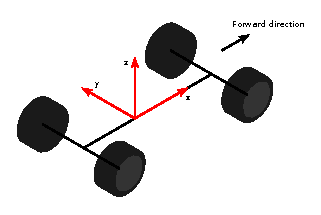
\includegraphics[width=0.5\linewidth]{0_Images/2_Introduction/BaseLinkFrame.eps}
    \captionof{figure}{The "base link" or "body" frame.}
    \label{Fig:BodyFrame}
\end{figure}

\begin{figure}
    \centering
    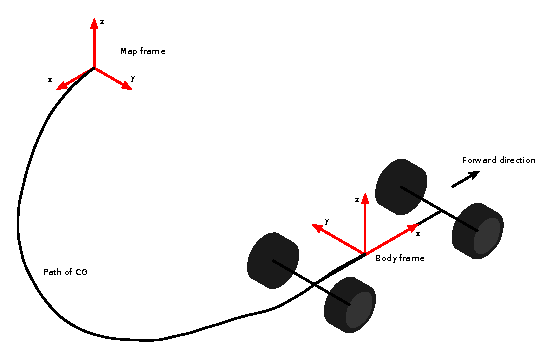
\includegraphics[width=0.5\linewidth]{0_Images/2_Introduction/MapAndBodyFrames.eps}
    \captionof{figure}{The map and body frames.}
    \label{Fig:MapAndBodyFrames}
\end{figure}

\begin{figure}
    \centering
    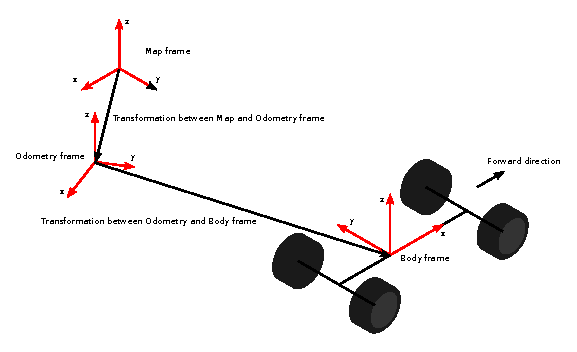
\includegraphics[width=0.5\linewidth]{0_Images/2_Introduction/MapOdomAndBodyFrames.eps}
    \captionof{figure}{The relationship between the map, odometry and body frames.}
    \label{Fig:MapOdomAndBodyFrames}
\end{figure}

Before leaving the realm of coordinate frames, one more must be mentioned. In the center of each wheel is defined a reference frame, here called the wheel frame. When the wheel is pointed straight ahead it has the same orientation as the body frame. This is illustrated in figure \ref{Fig:WheelFrame}. This frame will be important for talking about summing the forces from each wheel into one force and one torque on the CG. \\

Furthermore it is benefitial to name a few of the components of the race car. The main hoop is the bended rod around the drivers head that saves him or her from being crushed by the car if it should ever roll over. The snout is the rounded tip of the front of the car. The track of the car referes to the distance between the front and rear wheels along the x-axis, while the wheelbase refers to the distance between the right and left wheels along the y axis. These terms are illustrated in figure \ref{Fig:NameOfCarParts}.

\begin{figure}
    \centering
    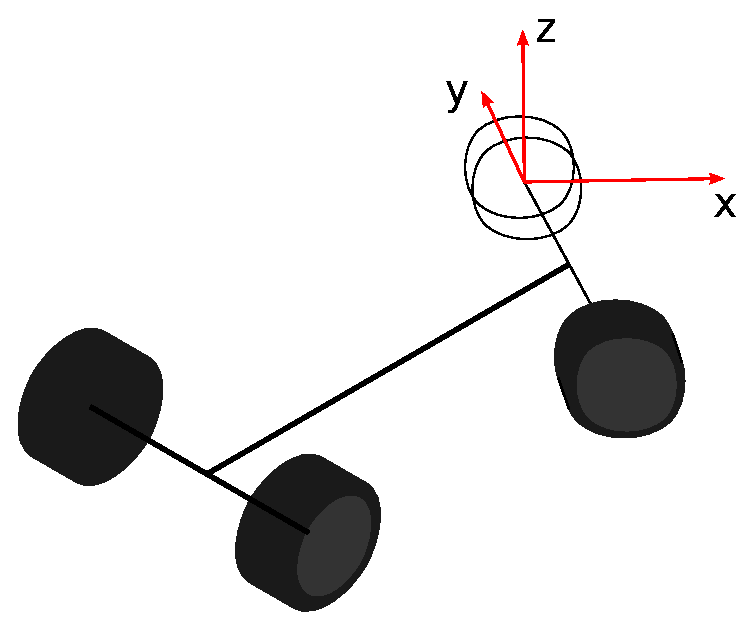
\includegraphics[width=0.5\linewidth]{0_Images/2_Introduction/WheelFrame.eps}
    \captionof{figure}{Front left wheel frame. There are similar ones in the other three wheels.}
    \label{Fig:WheelFrame}
\end{figure}


\begin{figure}
    \centering
    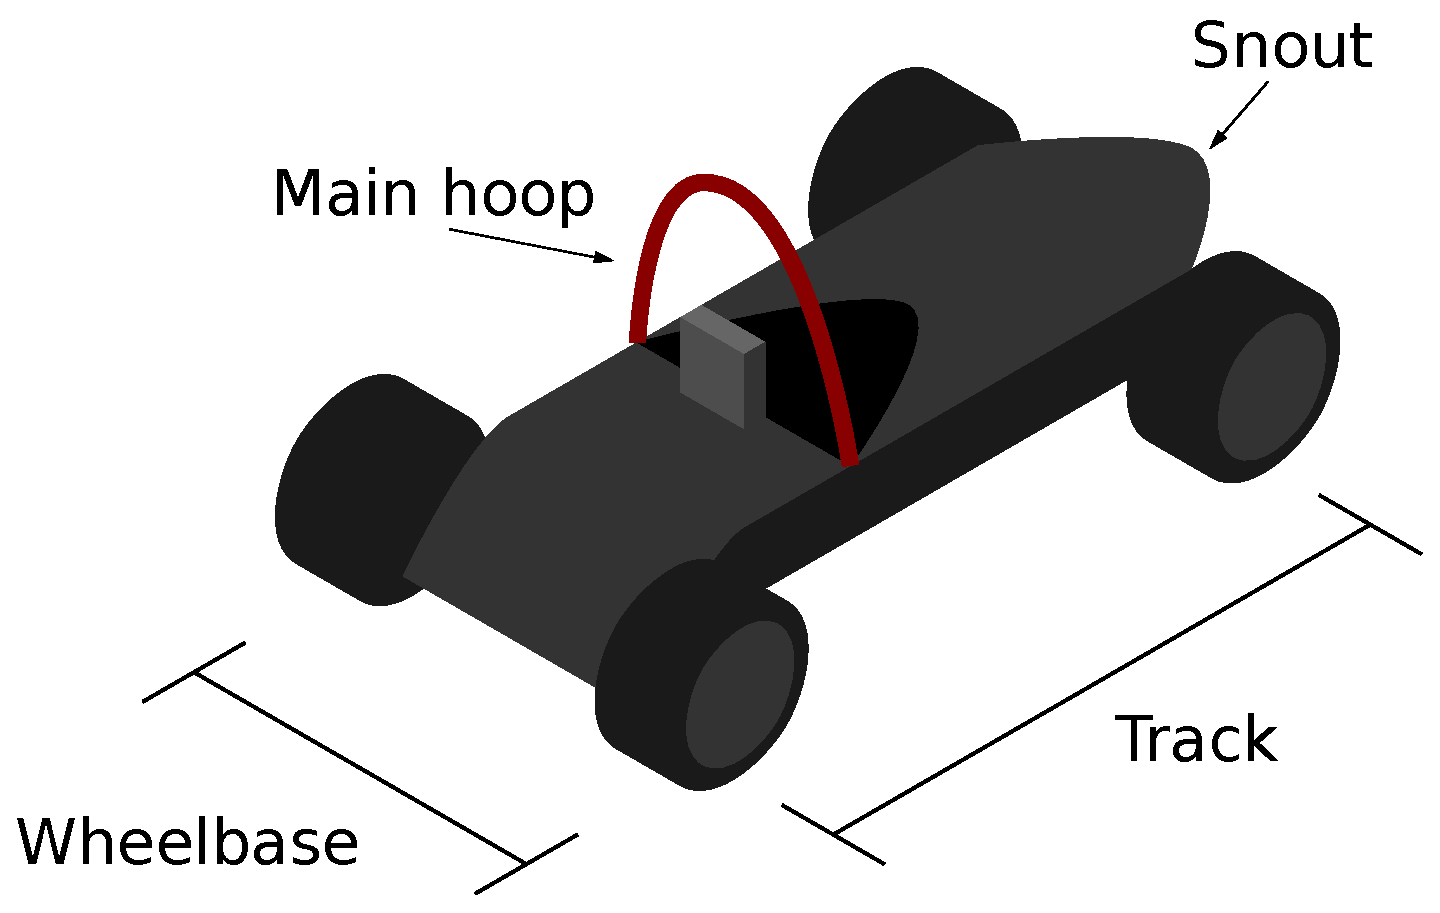
\includegraphics[width=0.5\linewidth]{0_Images/2_Introduction/NameOfCarParts.eps}
    \captionof{figure}{Simple model of the car with names of some parts, along with illustrations of track and wheelbase.}
    \label{Fig:NameOfCarParts}
\end{figure}

\section{Sensor theory}
The race car being used for this project deploys a high number of sensors, ranging from simple voltage meters on every other battery cell through ride height sensors and all the way to complex pieces of technology like the two LiDARs. For perception of the surroundings and understanding of the state of the car, the most relevant sensors are camera, LiDARs, IMU, INS, optical sensors and ride height sensors. Some of these needs a further explanation, and this is done in the below sections.

\subsection{LiDAR}
A LiDAR (light imaging, detection, and ranging) works by sending out light and timing how long it takes for the light to return. A typical LiDAR for autonomous vehicles has a rotating mirror that it sends an array of light beams at. This means the LiDAR covers an entire section of view, both horisontally and vertically. The resolution is set by how many channels it has vertically, how often it sends and receives light and the frequency of rotation. How far it can detect is determined by the sensitivity of the receiver and the strength of the sent beam. In a formula student application the allowed strength of the emited light is limited for safety reasons, which means the only real way of extending how far you can detect is by either increasing the sensitivity of your receivers photodetector or by increasing the number of vertical and horisontal channels. The latter will allow better outlier rejection, thus increasing how far you can detect. 

\subsection{IMU}
An Inertial Measurement Unit (IMU) measures acceleration and rate of change in rotation. It typically does so in all three dimension, amounting to a total of 6 degrees of freedom (DOF). Unless you're buying extremely expensive IMU's, it is typically going to be a MEMS (microelectromechanical system) type IMU. \par MEMS IMU's measure acceleration by having a microscopic mass attached to something elastic, so it's allowed to move in one dimension. When it is influenced by an acceleration parallel to its axis of movement, it will go in that direction. How far it moves is determined by the elasticity of the material, thus giving an indirect measure of how large the magnitude of the acceleration is. The IMU measures how much the mass has moved by a capacitance that changes with the movement of the mass. This is then converted to a measure of the acceleration along this dimension. The same is then done for the two other dimensions. \\ 

The rate of change in orientation is measured by the coriolis effect, which is the effect that a mass with a velocity in a rotating frame of reference will get an acceleration perpendicular to the velocity. A mass is made to vibrate back and forth, and when the accelerometer has a rate of rotation  with an axis perpendicular to the masses back and forth movement, it will get an acceleration perpendicular to the vibration axis. This is measured the same way as for the acceleration of the IMU. Since the way the IMU measures acceleration of the mass is restricted to one dimension, measuring the three possible dimensions of rotation demand three of these vibrating masses. \\

Since these sensors are so small, a high grade one being around the size of a box of matches, they are also noisy. The IMU on the race car therefore uses a Kalman filter and two GNSS antennas to filter away as much as possible of the noise. The output is still not good enough to use as a sole source of state estimation, as it drifts too quickly.
\subsection{Optical encoder}
To measure the angle of the steering wheel and the rate of rotation of the four wheels, optical encoders are used. They work by having a light source shine through holes in a disc mounted on the rotating part, centered on the axis of rotation. On the stationary part there are photodiodes, that send out a positive bit when the light hits them. The holes on the disc are made in a special pattern, such that the pattern of bits sent out by the photodiodes makes it possible to know at what angle the disc is currently in. This pattern typically employs a grey encoding to ensure that only one bit is changed each step. \\ 

A typical optical encoder, the ones used by Revolve NTNU included, has a stated accuracy of $\pm 10$ arcseconds, which equates to around $0.0028$ degrees. This is of course only under ideal circumstances, and does not take into acount effects such as concentricity of the glass disk on its hub, concentricity of the hub’s through bore relative to the optical disk, perpendicularity of the hub relative to the plane of the optical disk, parallelism of the optical disk face with the plane of the read head, thermal effects and so on. This is however much better accuracy than what is needed for our applications, as the error stemming from the optical encoder will be dominated by other errors. This are therefore deemed adequate.

\section{Sensor setup}
\subsection{LIDARs}
On board the car are two LIDAR's (light imaging, detection, and ranging). A Velodyne VL16 with 16 vertical channels and an Ouster OS1 with 64 vertical channels. \\ 

The Velodyne has a vertical resolution of $2.0\degrees$ spread across a $360\degrees$ field of view (FOV) and a horisontal resolution of $0.1$ degrees around the horizon and going down to $0.4\degrees$ towards the limits of it's vertical FOV, which is $\pm 15\degrees$. It's range measurmenents are accurate to $\pm 3 cm$, according to the manufacturer. \\

The Ouster has a vertical and horisontal resolution of $\pm0.01$ degrees, uniformly spaced around both it's horisontal FOV of $36\degrees$  and it's vertical FOV of $\pm 16.6\degrees$. It has a range resolution of $\pm 1.2 cm$. Both the LiDARS rotates at 20 Hz. \\

The OS1 is mounted in the hoop above the driver and scans $360\degrees$, while the VL16 is mounted in front of the front wheels, just in front of the snout of the car. The idea is that running them in parallel will increase the number of cones detected. \\

The placement of the LiDARs can be seen in figure \ref{Fig:SensorPlacementsV2}.

\iffalse
\begin{figure}
    \centering
    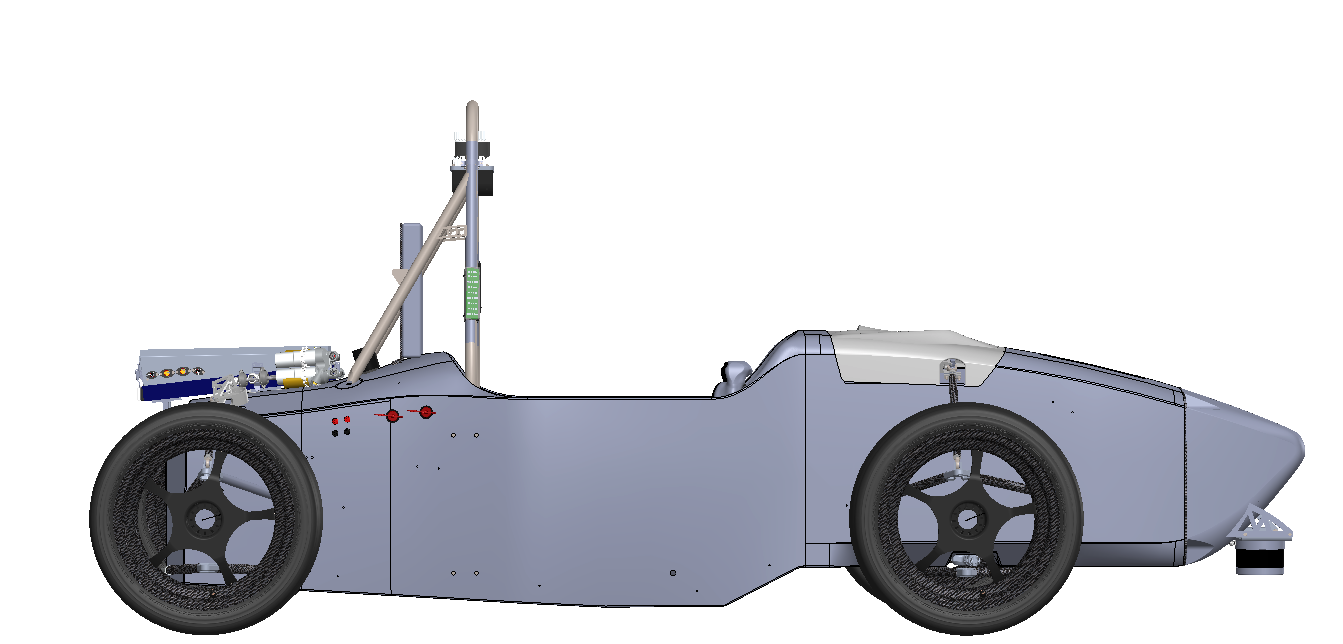
\includegraphics[width=0.8\linewidth]{0_Images/4_Implementation/LidarPlacements.png}
    \caption[Placement of the perception sensors.]
    {Placement of the perception sensors. A LiDAR and the camera are in the main hoop, while the other LiDAR is below the snout.}
    \label{Fig:SensorPlacements}
\end{figure}
\fi

\begin{figure}
    \centering
    
\includegraphics[width=0.8\linewidth]{0_Images/4_Implementation/SensorPlacements.eps}
    \caption[Placement of the perception sensors.]
    {Placement of the perception sensors. A LiDAR and the camera are in the main hoop, while the other LiDAR is below the snout.}
    \label{Fig:SensorPlacementsV2}
\end{figure}

\subsubsection{LiDAR detection algorithm}
The point cloud coming from the LiDARs get filtered based on position, where points too low, too high or too far away are discared. Then the ground is removed, by following the method used in \cite{GroundRemoval}. The point cloud is then downsampled into a voxel grid, and euclidian clustered, both using the PCL library \cite{PCL}. The true data in the downsampled clusters are then recreated and the centroid is found. Finally there is an outlier removal, where centroids with neighbors that are too close or too far away are removed. The centroids are then sent to the SLAM frontend as a set of detected cones.

\subsection{Camera}
For camera detection, a Basler PYTHON 1300 camera is placed in the main hoop(also shown in figure \ref{Fig:SensorPlacementsV2}), which is used for detection, as well as for determining the color of already detected cones. It has a 74.65 degree field of view and a resolution of 1280 x 1024, running at 200 Hz. \\

\subsubsection{Camera detection algorithm}
The images from the camera get fed into a neural net built on YOLO V3\cite{YOLOV3}. The last few layers of the net have been retrained on a quite extensive labeled dataset of cones, built up through the years by trading with other teams. This outputs bounding boxes on cones in the image, as well as the color of the detected cones. \\

The bounding boxes are then used to find the position in the body frame of the detected cones. Two methods have been tested for this. The first is using only geometry, considering the size and position of the bounding box. The second solution was to have the bounding boxes and the geometrically estimated positions sent into another neural net that corrects the initial estimate. This gave better results, the two errors in distance can be seen in figure \ref{Fig:rErrorCamera} and the error in angle in figure \ref{Fig:psiErrorCamera}.

\begin{figure}
    \centering
    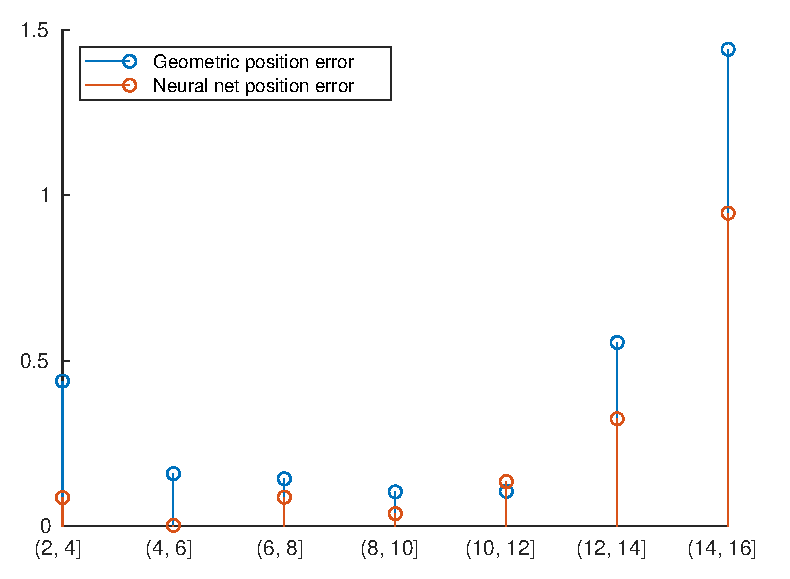
\includegraphics[width=0.8\linewidth]{0_Images/3_Theory/camDetection/rErrorCamera.eps}
    \caption[Error in the distance estimate of the two camera detection approaches.]
    {Error in the distance estimate of the two camera detection approaches.}
    \label{Fig:rErrorCamera}
\end{figure}

\begin{figure}
    \centering
    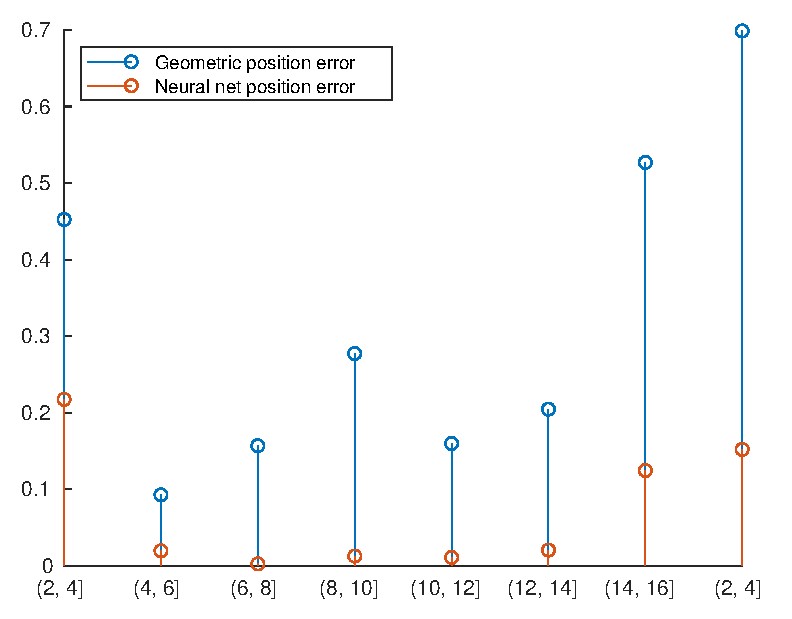
\includegraphics[width=0.8\linewidth]{0_Images/3_Theory/camDetection/psiErrorCamera.eps}
    \caption[Error in the angle estimate of the two camera detection approaches.]
    {Error in the angle estimate of the two camera detection approaches.}
    \label{Fig:psiErrorCamera}
\end{figure}

\subsection{INS}
The race car sports a Vectornav VN300 which is both an IMU as well as a GPS-receiver. It has a dual antenna setup where the two antennas are aligned with the x-axis of the car. This is done so it can get yaw angle, which the GPS gives out with 2 degrees of error. It outputs it's data at 400 Hz, and filters internally using a Kalman filter. \\ 

The INS outputs liner accelerations in 3 dimensions, the rate of change of the yaw, pitch and roll, as well as heading and a quite noisy position data from the GPS. \todo{Look over this, might want to rewrite whole subsection}

\subsection{Other}
Furthermore we have optical encoders giving us the RPM of each wheel. Another optical encoder measures steering wheel angle, which through a lookup table gives out the angle of the front wheels with the x-axis. There are also ride height sensors, that give the linear travel of the shock absorbers. This could indirectly give height above the ground, but in the authors opinion they are far from accurate enough to be usable.
\section{State estimation}
%\subsection{Previous work}
Nevn EKF, unscented particle filter, unscented EKF, classical approach, forskjellige papers som tar for seg deler av det vi ønsker å gjøre, men ikke alt. Nevn også at Automatica08 gjør nesten alt, men ikke gjør bank og inclination estimation, mens MainStateEst gjør alt unntatt yaw rate estimation, så vi ender opp med å snekre sammen begge disse. Nevn også at en del av arbeidet faktisk ikke blir gjort i de to direkte, men i imsland osv. Nevn også at EKF trenger mer tuning og mer beregningskraft. Muligens si det i neste subsubsection som en motivasjon for valg av approach. \\ 

State estimation in general usually referes to the following problem: Given a general nonlinear system 

\begin{equation}
    \Dot{x} = f(x,u(t), w(t))
\end{equation}

where $x$ is the state, $u(t)$ is the input at time $t$ and $w(t)$ is the noise input, and a nonlinear measurement function

\begin{equation}
    y = h(x,v(t))
\end{equation}

where $y$ is the measurement and $v(t)$ is measurement noise. In the specific case met by Revolve NTNU the states we want to approximate are the linear and angular velocities, which are then to be integrated up to give an initial estimate of the position, that is later to be corrected by SLAM. \\

The general field of state estimation is a broad one, that has been studied extensively. Below is detailed some general state estimation algorithms and design methodologies, as well as some that are more specific to our case. Some of the algorithms make more assumptions on the dynamical model, measurement function and the model and measurement noise, and thus it must be evaluated if it fits the specific problem at hand before it is chosen. \\

\subsection{Last years solution}

Last year this problem was solved by a rather rudiemental approach, colored by haste, as the team was scrambling to get everything else up and running for the first Revolve NTNU driverless car. It consisted of only using the RPM measurements from the wheels, taking the mean of them, multiplying with a constant estimate of the wheel radii to get the estimate of forward velocity $v_x$. The yaw rate was approximated by using the difference in the front wheel RPMs and the track width (see figure \ref{Fig:NameOfCarParts}).  \\ 

This very crude approximation gave ok results at very low speeds, but did not work at all at higher speeds, mostly because of wheel slip. The algorithm run on the same track at two different speeds can be seen in figure \ref{Fig:PureWheelOdom}, and clearly illustrates the degradation of performance at anything above very low speeds.   

\subsection{Kalman filter}

One could argue that the Kalman filter is the most widely used and most successfull algorithms to ever come out of the control comunity. It is ubiquitous, showing up in everything from cars to cell phones. What it is at its core is a way of combining sensor data and knowledge of a dynamical system, to get a better estimate of its states, even when faced with noise. \\ 

A kalman filter uses a dynamical model of a system, as well as knowledge of the noise that influences it, and is capable of combining several different types of sensors, making it a very powerfull and easy way of doing sensor fusion. It estimates how the system will develop, propagating not only its states, but also its covariance. This makes it able to know optimally how much it should give weight to measurements compared to the estimates coming out of integrating the dynamical model. \\ 

The kalman filter is said to be the optimal estimator when applied to a linear system, or a system that is linearized around it's true solution. The latter is of course not possible, since if we had the true solution we wouldn't need to estimate the states of the system. It does however mean that if we aren't far away from the solution, it will still be a good estimate. Doing so gives an extended Kalman filter\cite{EKF}, and is what is most used, considering most systems in the real world aren't truly linear systems. \\ 

To be more specific, the Kalman filter consists of a linear or linearized system with a transition matrix for each time step $k$, $F_{k}$, a way of influencing the system through the actuator $u_k$, represented as a matrix $B_{k}$. Together they give the apriori estimate of the state

\begin{equation}
    \hat{x}_{k|k-1} = F_k\hat{x}_{k-1|k-1} + B_k u_k
\end{equation}

To filter this, one propagates the covariance through the system, to find the predicted error covariance

\begin{equation}
    P_{k|k-1} = F_k P_{k-1|k-1} F^T_{k} + Q_k
\end{equation}

where $Q_k$ is the system noise covariance, and $P_{k-1|k-1}$ is the error covariance in the previous step. The error between the measured state $z_k$ and the estimated state $H_k \hat{x}_{k|k-1}$ is then found, where $H_k$ is the linear or linearized measurement function. Call this error $\Tilde{y}_k$. To find the optimal weighting between measurement and estimation, the so called Kalman gain, $K_k$, is created

\begin{equation}
    K_k = P_{k|k-1}H^T_kS^{-1}_k
\end{equation}

where 

\begin{equation}
    S_k = R_k + H_kP_{k|k-1}H^T_k
\end{equation}

is the measurement noise, $R_k$, plus the propagated noise from the previous step. This gain is then used to give a high weight to the measurement when the measurement noise is low and system noise is high, and vice versa. The estimate of the state then is

\begin{equation}
    \hat{x}_{k|k} = \hat{x}_{k|k-1} + K_k\Tilde{y}_k
\end{equation}

To set up for the next step, the a posteriori covariance is found by

\begin{equation}
    P_{k|k} = (I-K_kH_k)P_{k|k-1}(I-K_kH_k)^T + K_kR_kK^T_k
\end{equation}

This gives an error of 

\begin{equation}
    \Tilde{y}_{k|k} = z_k - H_k\hat{x}_{k|k}
\end{equation}

which can be proven to be optimal for linear systems and around the true trajectory of linearized nonlinear systems, as is done in e.g. in the original paper by Rudolf E. Kalman \cite{kalmanOG}.

\subsection{Advanced kalman filters}
There are extensions to the EKF, that gives better properties on some specific problems. One of the most applied of these is the Multiplicative Extended Kalman Filter (MEKF)\cite{MEKF}, and its derivations. It deals specifically with the problem of estimating the states of a 6DOF rotating rigid body in euclidian space. \\ 

The algorithm avoids some of the problems, like singularities, of dealing with attitude in a three-variable parametrization like Euler Yaw, Pitch, Roll, by working on a redundant parametrization for the attitude. This removes the singularities, but makes the state update a little more involved. The MEKF represents attitude as the product of an estimated attitude and the deviation from that attitude. Most implementations use a quaternion representation, leading to a product 

\begin{equation}
    q = \delta q(\phi)\oplus \Hat{q}
\end{equation}

where $\Hat{q}$ is the unit estimated quaternion and $\delta q(\phi)$ is a unit quaternion representing the rotation from $\Hat{q}$ to the actual attitude $q$, here parametrized by a vector, $\phi$, with three components. The choice of $\phi$ might vary, but usually the small angle approximation

\begin{equation}
    \delta q(\phi) = \begin{bmatrix} \phi / 2 \\ 1 \end{bmatrix} + \mathcal{O}(||\phi||^2)
\end{equation}

is used to get the correction on the estimate. The MEKF improves the stability properties of the EKF in attitude estimation by removing some singularities, but there is still room for improvement. A generalized MEKF is thus developed in \cite{GMEKF}, that gives a larger convergence region. \\ 

Another way of avoiding the problems of the three variable parametrization is an Additive Extended Kalman Filter (AEKF), which does the same thing, but through addition of quaternions instead. This has however been proven to be equavivalent to the MEKF\cite{AEKF}, and is thus not discussed further. \\

Yet another extendsion of the EKF is the Unscented EKF\cite{UKF}. Instead of linearizing the nonlinear state transition function to be able to propagate the covariance, like the EKF does, it uses what is called an Unscented Transformation\cite{UTrans}. This means that instead of assuming that the first order approximation to the nonlinear function is good enough and discarding the rest of the information it can give us, it approximates the state probability distribution by a set of discrete points, called Sigma points. These and the mean are then propagated through the full nonlinear state transition function. This gives a new predicted mean and the propagated sigma points are used to approximate a new distribution in the transformed space, usually a Gaussian. \\

The points chosen are carefully picked to perfectly represent the mean and covariance of the original distribution, and thus it is proven to give a third order approximation of the propagated distribution for a nonlinear state transition with additive white noise, compared to only a first order approximation in the EKF. For a nongaussian distribution this method is still correct to the second order.\\ 

One update step of the UKF consists of finding a set of sigma points, $x_{k,i}$, from the original distribution and a set of weights, $w_i$, as follows

\begin{alignat*}{3}
    & x_{k-1,0} &&= \Bar{x_k} \\
    & x_{k-1,i} &&= \Bar{x_k} + (\sqrt{(N+\lambda)P_{x,k}}_i, i &&= 1,...,N \\
    & x_{k-1,i} &&= \Bar{x_k} - (\sqrt{(N+\lambda)P_{x,k}}_{i-N}, i &&=N + 1,...,2N \\
    & w_{k-1,0}^{(m)} &&= \lambda/(N+\Lambda) \\ 
    & w_{k-1,0}^{(c)} &&= \lambda/(N+\lambda) + (1-\alpha^2 + \beta) \\
    & w_{k-1,i}^{(m)} &&= w_{k-1,i}^{(c)} = 1/(2(N+\lambda)), i &&= 1,...,2N
\end{alignat*}

where $\lambda = \alpha^2(N+\kappa) - N$ is a scaling parameter. $\alpha$ determines the spread of the points around the mean and is usually set to a small positive value (e.g. 0.001). $\kappa$ is a secondary scaling parameter which is usually set to 0, and $\beta$ is used to incorporate prior knowledge about the distribution ($\beta=2$ is optimal for the Gaussian distribution). $P_{x,k-1}$ is the covariance of $x$ at time $k-1$, and N is the number of state space dimensions. \\

These points are sent through the nonlinear function, giving a set of new points $y_{k-1,i}$. The new points are then used with the weights to give the new mean and covariance matrix of the new points. 


\begin{equation}
    \Bar{y}_{k-1} \approx \sum_{i=0}^{2N} w_{k,i}^{(m)}y_{k-1,i}
\end{equation}

\begin{equation}
    P_{k-1, yy} \approx \sum_{i=0}^{2N} w_{k,i}^{(c)}(y_{k-1,i} - \Bar{y})(y_{k-1,i} - \Bar{y})^T
\end{equation}

To find the Kalman gain, one also need the covariance of the old state with the new, 
\begin{equation}
    P_{k-1, xy} \approx \sum_{i=0}^{2N} w_{k,i}^{(c)}(x_{k-1,i} - \Bar{x})(y_{k-1,i} - \Bar{y})^T
\end{equation}

and the covariance of the old state with itself,

\begin{equation}
    P_{k-1,xy} \approx \sum_{i=0}^{2N}w_{k,i}^{(c)}(x_i - \Bar{x})(x_i - \Bar{x})^T
\end{equation}

All that remains then is to incorporate measurements. To do this one creates the Kalman gain, $K$, much like with the EKF, and use this to weight between the measurement and the estimate.

\begin{equation}
    K_k = P_{k-1,xy}P_{k-1,yy}^{-1}
\end{equation}

This then gives us the posterior estimated state

\begin{equation}
    x_k = x_{k-1} + K_k(z_k - \Bar{y}_{k-1})
\end{equation}

where $z_k$ is the measured state, $\Bar{y}_{k-1}$ is the a priori estimate of the state and $x_{k-1}$ was the previous a posteriori estimate. To the get new state covariance matrix is then simply

\begin{equation}
    P_k = P_{k-1,xx} - K_kP_{k-1,xy}K_k^T
\end{equation}

Although this seems more complicated, it actually is of the same computational order of magnitude as the EKF, and gives a much better approximation.

\subsection{Particle filter}
Another solution to the state estimation problem is the Particle Filter, first introduced in \cite{ParticleFilter} in 1996, but not made viable before 2000, when resampling was introduced\cite{ParticleResampling}. It attacks the problem of state estimation from the view point that the best estimate of the state could be gotten if we had the probability density function of the state given the inputs, measurements and measurement model. But since this is not something we usually have analytically, it instead approximates it by a discrete set of particles, where the density of the particles in the state space over time will approximate the true pdf. \\

The basic principle of a particle filter is 

\begin{itemize}
    \item pulling samples (usually called particles) from a prior distribution, 
    \item weighting them with how much deviation there is from the true distribution, 
    \item normalizing the weights and then resampling the particles (with replacement) where the probability of sampling a specific particle is its weight. 
\end{itemize}

In a state estimation setting this means starting with N particles, distributed in some manner around the state space (usually uniformly). Then every step, $k$, in the particle filter the particles $\{x_{k-1,i}\}$ are propagated according to the state transition function

\begin{equation}
\forall i, \; \; x_{k,i} = f(x_{k-1,i}, u_k)
\end{equation}

where $u_k$ is the input at that step. Here some have had good results with adding some noise to the propagation, in order to speed up exploration of the state space\cite{ParticleNoise}. The weighting function, $p(z_k|x_{k,i})$, is the probability of observing the measurement, $z_k$, given the state. This function is given by the measurement model for the different sensors. In the case of additive gaussian noise on a single sensor with linear measurement function, this is simply

\begin{align}
    p(z_k| & x_{k-1, j}, u_k) \propto \\
    & exp(-1/2(z_k - Cf(x_{k-1, j}, u_k))^T
    (\Sigma_v + C\Sigma_wC^T)^{-1}(z_k - Cf(x_{k-1, j}, u_k))) \nonumber
\end{align}

Where $\Sigma_v$ is the process noise covariance and $\Sigma_w$ is the measurement noise covariance. \\ 

One can also use more heuristic approaches, like using the euclidian distance as the weighting function, normalized to one. This was employed in the particle filter Revolve NTNU uses for path planning. There the weighting of the different center line hypotheses is a function of the sum of the cones' deviations from the mean track width and has given good results.

\subsection{Visual odometry}

A less classical approach to state estimation is Visual Odometry (VO). It exists in many variants, but the main principle is finding correspondences between successive image frames, using geometric considerations on these points or regions to estimate the relative change in pose between the two frames. This gives the change in pose, which can then be summed to give the pose relative to the initial pose, as well as derivated to get an approximate velocity and angular rate.\\ 

One of the most popular algorithms is SVO\cite{SVO} and more recently its stereo extension SVO 2.0\cite{SVO2}. It finds feature points in the two images using FAST corner detection\cite{FAST} and Edgelets egde detector\cite{Edgelet}. Only the points that can be matched between the images are kept. Around the features a patch of pixels are chosen. These patches are then reprojected from one of the frames into the other to find the pose that minimizes photometric error between the reprojection and the true pixels, se figure \ref{Fig:SVO}. \\

\begin{figure}
    \centering
    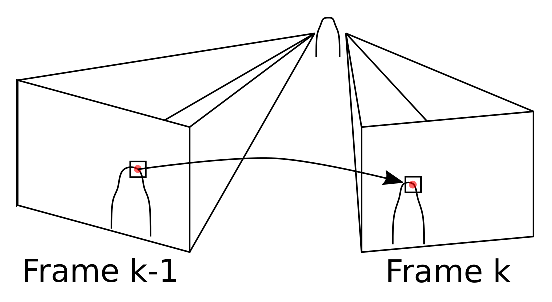
\includegraphics[width=0.8\linewidth]{0_Images/3_Background/SVO.eps}
    \caption[Illustration of SVO's reprojection of an image patch.]
    {Illustration of SVO's reprojection of an image patch. It tries to find the pose that minimizes the photometric error between the pixels projected into the frame and the pixels they get projected onto.}
    \label{Fig:SVO}
\end{figure}

A problem with using one single camera for positioning, is that the two scenes can look identical in the two images, but be of completely different scale. Without stereo information, the camera doesn't give information about scale, thus rendering the positioning information quite useless. This is tackled by either having something in the frame that you know the size of that everything else can relate to, or, as in the case of SVO 2.0, by using two cameras with a known transformation between. This gives gives the scale information needed. \\

SVO and SVO 2.0 are implemented in c++ and publicly available under a non-commercial license. \\

Another viable algorithm is DSO\cite{DSO}. It looks at entire regions of pixels where the pixel intensity gradients are large enough, samples pixels randomly from the regions and tries to find the pose that minimizes the photometric error of the reprojected pixels. \\

The author of the original paper has a publicly available c++ implementation, but although there is a theoretical stereo extension called DSO-Stereo\cite{DSOStereo}, the only implementations of the algorithm that are publicly available is a very unstable one from someone other than the author. \\

Yet another option is ORB-SLAM2\cite{ORBSLAM}, which uses ORB features\cite{ORB} to find point correspondences in two consecutive frames. This gives an initial estimate on the change in position between the frames, as well as distance measurements of different features. It then uses this information to do full SLAM, building a 3D map of points and placing the camera in that map (more on SLAM below). By ignoring the information about the map this is effectively a state estimator as well. ORB-SLAM2 works on a stereo setup and a implementation by the authors is publicly available.

\subsection{Lidar Odometry}

Instead of using the camera information to get a visual odometry, one could apply the same set of ideas to the point cloud coming out of the LiDARs. This gives what is known as LiDAR Odometry. \\ 

The most known, publicly available, algorithm at the moment is LOAM\cite{LOAM}. It, much like ORB-SLAM, finds feature points that it can match in successive swipes of the LiDAR, that then gives point to point distance estimates. These distance estimates are then added iteratively to a set of distances, a single step of a nonlinear optimizer tries to find the pose change between frames. Distance estimates are added untill the optimization step converges. \\

A very recent development is DeepLO\cite{DeepLO}, where they use neural nets, with both supervised and unsupervised training to achieve very good performance on the KITTI dataset. There is however, as of now, no code open to the public.

\subsection{Nonlinear observer}
\iffalse
One of the first papers to treat nonlinear observer design by errorlinearization was \cite{FirstErrorLinNonlinObs}. \\

The first type that should be mentioned is EKF, statisctically motivated. \\ 

Explain the general problem, maybe mentioning stuff like observability, different forms of stability of the observers and especially the convergence to the true value over time. \\

Different types of nonlinear observers that are benefitial to mention

\begin{itemize}
    \item Observers derived by linear approximation (maybe EKF first?)
    \item Statistically motivated expanded degree observers like EKF
    \item Observers derived by error linearization
    \item High gain observers
    \item Minimum energy?
    \item Sliding mode observers?
    \item Before arriving at the main one: Observers derived through Lyapunov analysis
\end{itemize}
\fi

The term nonlinear observer refers to any dynamical system run in parallel with a dynamical system, where some or all of the internal states of the nonlinear observer tries to match some or all the states of the original dynamical system. There are mountains of different nonlinear observers, as this is a very general term. \\ 

To separate the different types of observers, it is benefitial to do so by how they have been derived. This makes it possible to talk about each class' general properties, their pros and cons, especially in regards to ease of derivation for a specific system, how much tuning there is and overall performance.

\subsubsection{Linear approximation}

The first that should be mentioned is the nonlinear observers derived by linear approximation of the dynamical system it is trying to represent\cite{LinearizingNonlinObs}. If this is done for a linear system 

\begin{align}
    \Dot{x} &= Ax + Bu \\
    y &= Cx
\end{align}

the resulting observer

\begin{align}
    \Dot{\hat{x}} &= A\hat{x} + Bu + L(y - \hat{y}) \\
    \hat{y} &= C\hat{x}
\end{align}

will give exponential convergence of the estimate, $\hat{x}$, to the true state, $x$, as long as $A-LC$ is Hurwitz\cite{Hurwitz}. In the case of a nonlinear system the A's, B's and C's will be the first order approximations

\begin{equation}
    A = \frac{\partial f}{\partial x}|_{x=x_0}
\end{equation}
\begin{equation}
    B = \frac{\partial f}{\partial u}|_{x=x_0}
\end{equation}
\begin{equation}
    C = \frac{\partial h}{\partial x}|_{x=x_0}
\end{equation}

where again $f$ is the state transition function and $h$ is the measurement function. This will however only give local asymptotic stability when the $A-LC$ is Hurwitz and the pair $\{A,C\}$ is observable. Many of the relevant dynamical systems do not have this property, nor is local asymptotic stability always enough, so the research community searched on for more sophisticated solutions with better properties. 

\iffalse
One of the next steps the community took was to develop the statistically motivated methods, most prominent and succesfull of which is the Extended Kalman filter. These methods are typically so-called expanded order observers, meaning they have more internal states than the system that it is trying to approximate the states of. In the case of the Kalman filter these internal states are $\{\hat{x},P\}$, which illustrates usual approach taken by these methods; to approximate not only the state of the system, but also the underlying probability distribution it comes from. 
\fi

\subsubsection{Error linearization}

A rather large theoretical step forward was taken by Krener and Isidori\cite{FirstErrorLinNonlinObs}, when they developed a nonlinear observer by so-called error linearization. The idea is to find transformations of the state and output coordinates, 

\begin{equation}
    z = \Theta(x)
\end{equation}
\begin{equation}
    w = \gamma(y)
\end{equation}

such that nonlinear system can be expressed in the form

\begin{align}
    \Dot{z} &= Az + \alpha(u,y) \\
    w &= Cz + \beta(u,y)
\end{align}

This makes it easy to make an observer for the system

\begin{align}
    \Dot{\hat{z}} &= A\hat{z} + \alpha(u,y) + L(w-\hat{w}) \\
    \hat{w} &= C\hat{z} + \beta(u,y) \\
    \hat{z}(0) &= \Theta(\hat{x}^0) \\ 
    \hat{x} &= \Theta^{-1}(\hat{z})
\end{align}

If the pair $\{C,A\}$ is observable and one has placed the spectrum of $A-LC$ in the open left half plane, then this observer will converge exponentially. \\

The problem is of course that not many systems are possible to transform like this, and many who do can only be transformed into this form by repeated derivations of the output. The latter makes the whole design very vulnerable to noise, in fact so much that it has little practical use. \\

\iffalse
A similar approach is the so called High Gain Observer\cite{HighGain}, which gets the system into the uniformly observable form, and then adds a error term of $L(y-\hat{y})$ to each state. If the gain is large enough this can be proven to be locally asympotically stable, but it suffers from the same problems as the error linearization. \\
\fi

\subsubsection{Nonlinear observers designed using Lyapunov analysis}

A more recent developement, spearheaded in part by the research community here at NTNU, is the use of Lyapunov anaysis to develop nonlinear observers that converge asymptotically to the true state\cite{PassiveFossen}. Made first for Dynamic Positioning (DP) of large boats, it consists of starting out with an initial guess for an observer, then trying to prove it's stability by Lyapunov analysis and then modifying the observer until stability can be proven. \\

By Lyapunov analysis\cite{Lyapunov} is meant the process of finding a Lyapunov function candidate $V(\Tilde{x})$ that is positive definite, i.e. larger than or equal to zero for all $x\neq \Vec{0}$. Here $\Tilde{x}$ is the error between the true state and the estimate. The proof is then to show that this function has the special property that

\begin{equation}
    \frac{dt V(\Tilde{x})}{dt} \leq 0 \;\; \forall \hat{x}
\end{equation}

If such a Lyapunov function can be found and this property holds, then the error will always go asymptotically to zero and the observers works as desired. Other properties as also possible to derive with slight changes to the analysis formulation, but this is the main way it is used. \todo{Double check math here and consider rewriting} \todo{Maybe add parts about I/O stability proofs and GES?}. \\

One of the main reasons for choosing a nonlinear observer over a Kalman filter is that once the observer is developed it needs much less tuning than the Kalman filter. An example is the 120 covariance equations in the Kalman filter for the supply vessel discussed in \cite{PassiveFossen}, compared to the 17 gains in the nonlinear observer. Another huge benefit compared to the EKF is global asymptotic stability and sometimes global exponential stability, compared to only local symptotic stability of the EKF. \\ 

For a system of the form 

\begin{align}
    \Dot{x} &= f(x,u,v) \\
    y &= h(x,u,w)
\end{align}

where $x$ is the state, $u$ is the input and $v$ and $w$ are noice inputs, a good place to start for the observer design would be to simply copy the dynamics with a proportional error term, setting the noise to zero.

\begin{align}
    \Dot{\hat{x}} &= f(\hat{x}, u, 0) + K\Tilde{y} \\
    \hat{y} &= h(\hat{x}, u, 0)
\end{align}

Here $\Tilde{y} = y -  \hat{y}$ is the difference between the measured y and the estimated y. A first guess for the Lyapunov function could then be the difference in physical energy of the system when in the true state and when in the estimated state, or the quadratic sum of the error in the estimated states. 
\section{SLAM}

Simultaneous Localization And Mapping (SLAM)\cite{FirstSLAMMention}\cite{SLAMIntro} refers to both the problem and the algorithms that tries to solve it. The problem is to incrementally build a map of landmark observations, while also locating the agent which observes these measurements in the map. Popular solutions to this include EKF-SLAM\cite{EKFSLAM}, FastSLAM\cite{FastSLAM} and factor graph\cite{Dellaert} solutions like iSAM2\cite{iSAM2}. These solutions are explained in detail below. \\

The problem is usually formulated probabilistic. The important variables used in the formulation are the following:

\begin{itemize}
    \item $x_k$: The pose of the agent at time $k$. 
    \item $u_k$: The vector of inputs that move the agent to the pose $x_k$ at time $k$.
    \item $m_i$: A vector containg the location of the $i$th landmark in the map frame. 
    \item $z_k$: A vector of all the measurements of the relative positions of landmarks that can be measured from the agent at time $k$ 
\end{itemize}

There is also a number of sets that are needed

\begin{itemize}
    \item $X_{0:k} = \{x_0,x_1,...x_k\} = \{X_{0:k-1},x_k\}$: The history of all the agents poses.
    \item $U_{1:k} = \{u_1,u_2,...,u_k\} = \{U_{1:k-1},u_k\}$: The history of all control inputs.
    \item $m=\{m_1,m_2,...,m_n\}$: The set of all landmarks, also called the map.
    \item $Z_{1:k}=\{z_1,z_2,...,z_k\} = \{Z_{1:k-1},z_k\}$: The set of all landmark observations that have been measured until time $k$.
\end{itemize}

The problem can now be formulated as computing the probability distribution 

\begin{equation}
    P(x_k,m|Z_{0:k},U_{0:k},x_0)
\end{equation}

at every time step $k$. This is the joint posterior density of location of all landmarks in the map and the agents pose, given all the measurements that have been seen so far and the control inputs that have been applied to the agent. \\

One usually wants to compute this distribution reccursively. This is done by using the previously computed distribution $P(x_{k-1},m|Z_{0:k-1},U_{0,k-1},x_0)$ at the previous time step $k-1$, together with a model for the next pose of the agent given the current input and pose, 

\begin{equation}
    P(x_k|x_{k-1},u_k)
\end{equation}

and a measurement model, giving the probability of making an observation $z_k$ when both the agents pose and the landmarks location is known

\begin{equation}
    P(z_k|x_k,m)
\end{equation}

The standard way of doing it now is doing a two part update of to get the desired distribution. First a time update, that uses the motion model to find an estimate for the agents location


\begin{align}
    P(x_k,m|Z_{0:k},U_{0:k}, x_0) 
     = & \int P(x_k|x_{k-1},u_k) \\
    & \times P(k_{k-1},m|Z_{0:k-1},U_{0:k-1},x_0)dx_{k-1}
\end{align}

The second update is to include the effect of measurements, 

\begin{equation}
\begin{split}
    P(x_k,m|Z_{0:k},U_{0:k},x_0) 
    = \frac{P(z_k|x_k,m)P(x_k,m|Z_{0:k-1},U_{0:k},x_0)}{P(z_k|Z_{0:k-1},U_{0:k}}
\end{split}
\end{equation}

How the method describes the motion model and measurement model, and how it does the two updates differ from method to method, but this is the main idea that lies behind them all. The SLAM problem has been said to have been solved, but this is only meant theoretically; in practice there are still problems with all of the methods. The main challenges that are still not overcome completely are 

\begin{itemize}
    \item How to update in real time.
    \item How to build a consistent map that doesn't make the computational demand grow exponentially.
    \item How to associate measurements to landmarks.
\end{itemize}

\subsection{EKF}

One of the first solution to the SLAM problem was the EKF-SLAM\cite{EKFSLAM}. It assumes a motion model 

\begin{equation}
    P(x_k|x_{k-1},u_k) \iff  x_k = f(x_{k-1},u_k) + w_k
\end{equation}

where $f(x_{k-1},u_k)$ is the model of the vehicle kinematics and $w_k$ is additive, zero mean, uncorrelated Gaussian noice with covariance $Q_k$. The observation model is similarily assumed to be 

\begin{equation}
    P(z_k|x_{k-1},m) \iff  z(k) = h(x_{k},m) + v_k
\end{equation}

where $h$ is a function describing the geometry of the observations and $v_k$ is additive, zero mean, uncorrelated Gaussian noise with covariance $R_k$. \\

Using the above models, the standard EKF can be used to compute the mean 

\begin{equation}
    \begin{bmatrix} \hat{x}_{k|k} \\ \hat{m}_k \end{bmatrix} = E[\begin{bmatrix} x_k \\ m \end{bmatrix} | Z_{0:k}]
\end{equation}

and the covariance

\begin{align}
    P_{k|k} &= \begin{bmatrix} P_{xx} & P_{xm} \\ P^T_{xm} & P_{mm} \end{bmatrix} \\
     &= E\bigg[\begin{bmatrix} x_k-\hat{x}_k \\ m - \hat{m}_k\end{bmatrix}\begin{bmatrix} x_k-\hat{x}_k \\ m - \hat{m}_k\end{bmatrix}^T \bigg| Z_{0:k} \bigg]
\end{align}

of the desired joint posterior distribution $P(x_k,m|Z_{0:k},U_{0:k},x_0)$. This is done by first time-updating using

\begin{align}
    \hat{x}_{k|k-1} &= f(\hat{x}_{k-1|k-1},u_k)
    P_{xx,k|k-1} &= \nabla f P_{xx,k-1|k-1}\nabla f^T + Q_k 
\end{align}

Here $\nabla f$ is the jacobian of f at the previous estimate $\hat{x}_{k-1|k-1}$. The landmarks aren't updated, since they are assumed stationary. The measurement update is then

\begin{align}
    \begin{bmatrix} \hat{x}_{k|k} \\ \hat{m}_k \end{bmatrix} &= 
    \begin{bmatrix} \hat{x}_{k|k-1} \\ \hat{m}_{k-1} \end{bmatrix}
    + K_k[z(k) - h(\hat{x}_{k|k-1},\hat{m}_{k-1}] \\
    P_{k|k} &= P_{k|k-1} - K_kS_kK_k^T
\end{align}

where the innovation, $S_k$, is defined as

\begin{equation}
    S_k = \nabla hP_{k|k-1}\nabla h^T + R_k
\end{equation}

and the Kalman gain, $K_k$, is defined as

\begin{equation}
    K_k = P_{k|k-1}\nabla h^T S_k^{-1}
\end{equation}

Here $\nabla h$ is the jacobian of h computed at $\hat{x}_{k|k-1}$ and $\hat{m}_{k-1}$. \\

This solution to the SLAM problem has been proven to converge if the motion model and measurement model is correct. It does however suffer from a quadratically growing complexity in the number of landmarks, and will not be possible to implement in real time if the total map size gets too big. It also is very sensitive to incorrect associations between measurements and landmarks and since it is a linear approximation to the true model, it has the same problems that the EKF does in terms of divergence from the true solution. 

\subsection{FastSLAM}

Theoretically, one could use a particle filter\cite{ParticleFilter} to solve the SLAM problem. But practically, the particle filter can't deal with the high dimensionality of the state space, making it computationally unfeasible without any modifications. One such modification is the Rao-Blackwellized Particle Filter (RBPF)\cite{RBPF}. It assumes it's possible to partition the state, $\xi$, into two states, $\xi_1$ and $\xi_2$, that has a joint probability distribution 

\begin{equation}
    P(\xi_1,\xi_2) = P(\xi_2|\xi_1)P(\xi_1)
\end{equation}

where the conditional probability $P(\xi_2|\xi_1)$ is possible to represent analytically. This means that only $P(\xi_1)$ needs to be represented by sampling particles. The effect of this is that the marginal $P(\xi_2)$ is possible to compute with less particles, greatly reducing the computational complexity. \\

Applying this mindset to the SLAM problem results in what is known as FastSLAM\cite{FastSLAM1}. The idea is that since the error in landmarks will all depend on the error in pose, the pose is the only variable in $\xi_1$. The remaining set of variables, $\xi_2$, is then the map, which is found by conditioning on the state and the measurements. This leads to the following factorization of the joint distribution

\begin{equation}
    P(X_{0:k},m|Z_{0:k},U_{0:k},x_0) = P(m|X_{0:k},Z_{0:k})P(X_{0:k}|Z_{0:k},x_0)
\end{equation}

Furthermore, it is assumed that the landmarks are independent of each other, i.e. that the joint landmark distribution $P(m|Z_{0:k},x_0)$ can be written as the product of each landmarks distribution

\begin{equation}
    P(m|X_{0:k},Z_{0:k}) = \prod_{1<i<n}P(m_i|X_{0:k},Z_{0:k})
\end{equation}

The method then employs $R$ particles, that each represent a pose, calculated by using a normal particle filter by propagation using a motion model, weighting using the measurement model and resampling. Each particle has a map, that is calculated analytically by the particle trajectory, measurements and the measurement model. This is the same as saying that each particle has a set of $n$ small EKFs, that each try to estimate the position of each landmark. \\

The independence assumption between the landmark distributions mean that the complexity of the computations can be kept to $Rlog(n)$, compared to $n^2$ of the EKF-SLAM. \\

There are two different version of FastSLAM: FastSLAM 1.0\cite{FastSLAM1} and FastSLAM 2.0\cite{FastSLAM2}. The difference lies in the proposal and weighting functions. \\

FastSLAM 1.0 uses the motion model 

\begin{equation}
    x_{k,i} ~ P(x_k|x_{k-1,i},u_k)
\end{equation}

as a proposal function, which gives that the weights are calculated using the marginalized observation model

\begin{equation}
    w_{k,i} = w_{k-1,i}P(z_k|X_{0:k,i},Z_{0:k-1})
\end{equation}

For FastSLAM 2.0 however, the proposal function uses the latest observation $z_k$,

\begin{align}
    x_{k,i} &= P(x_k|X_{0:k-1,i},Z_{0:k},u_k) \\
    &= \frac{1}{C}P(z_k|x_k,X_{0:k-1,i},Z_{0:k})P(x_k|x_{k-1,i},u_k)
\end{align}

Where C is a normalizing constant. This gives that the importance weights are calculated as

\begin{equation}
    w_{k,i} = w_{k-1,i}C
\end{equation}

According to \cite{SLAMIntro} this leads to a weighting function that is locally optimal. This means that it gives the smallest posible variance in the weight $w_{k,i}$, given $X_{0:k-1,i}$, $Z_{0:k}$ and $U_{0:k}$.

\subsection{Factor graphs}

Talk about bayesian networks, how they're nice for representing the problem but unfit for doing the optimization. Talk about the graphical extension to bayesian networks that factor graphs are, how they solve the problem and how they represent all the different data. Maybe also a part about how they allow us to do optimization on only a small part of the problem at a time. \\ 

Mention loop closures. Should there be a part about how we do loop closures?? I think so. \\

Talk about how since we are doing featureless SLAM we need some sort of front end doing data association, so it transitions well into the next section about data association.

\subsection{iSAM}


\section{Data association}

When using factor graphs to solve the SLAM problem, an important thing to think about is how the measurements are associated to the right landmark. This is relatively easy when you do feature-based SLAM, e.g. when you use a visual slam system like ORB-SLAM \cite{ORBSLAM}. This is because the measurement itself has a direct way of being compared with other features for how alike they are, and a single point in space is usually pretty distinct. \\

This is however not the case with the detection systems employed on Revolves race car. Since the cones are very similar, a feature extracting algorithm was not thought to work, and all the detections systems only give out a position in the plane, with the camera system outputting a cone color as well. This means the SLAM system needs to be able to keep track of which measurements are to the same cone, or landmark as it's usually referred to when talking about SLAM. \\

\subsection{Last years solution}

Last year this was done with a very naive algorithm, that simply said that if a new detection was within a certain radius from an existing cone in the exisitng map, it was the same cone. If a measurement could not be associated to the existing map, it had to be seen above a certain number of times to be added to the map. This meant that the system had a list of hypothesises that a new measurement was associated to the same way it was associated to the map. \\ 

This method did however not take into account the different spatial uncertainties stemming from the different detection algorithms, nor did it account for the varying uncertainty of the state estimation. It also didn't have a way of distrusting the landmarks if it hadn't been seen when it should have been. \\

\subsubsection{Previous work} \todo{Remove title previous work?}

Most of the work done on data association is used for object tracking, typically using a radar\cite{RadarTracking}, but also more recently been used to track visually\cite{VisualTracking}. Data association used for tracking implies finding out which of the tracked objects correspond to new measurements, where typically the measurements are all made from a stationary vantage point, while the objects are moving around. This means one must predict where the objects are going to be and try to match all observed objects with objects that are being tracked. \\

Data association applied to SLAM have been more common in the recent years. It is an almost opposite problem to the tracking problem, as the observer is the one moving around, while the landmarks are standing still. While a lot of the work done on tracking focuses on single or a handfull of objects to track, when solving the SLAM problem one by definition want to be able to handle a large amount of landmarks. This is because the output of the system is going to be the map, and you want it to be able to handle all the landmarks that build up the map. The data association problem met in the two settings are however quite similar, and work done in one field therefore benefits the other. \\

\subsection{Nearest Neighbour}

When talking about the data assocation problem and its solutions it's essential to keep in mind at all times what application is being discussed. In many of the earlier cases the tracking problem is simply matching measurements with one object, in which case a nearest neighbor matching with the Malahanobis distance can work wonders\cite{ShalomTracking}. \\ 

In this case it is assumed that one of the measurements is the object, and you're simply trying to know which one it most likely is. It's assumed that the objects movement can be approximated as

\begin{equation}
    p_{next} = Ap_{prev} + w_{model}
\end{equation}

That is then measured with a measurement model

\begin{equation}
    p_{meas} = Hp_{true} + w_{meas}
\end{equation}
 
Here A is the linearized dynamic model for how the object moves, H is the linearized measurement function and $w_{model}$ and $w_{meas}$ are additive zero-mean white noise for the model and measurement, respectively. It then uses a Kalman filter step to propagate the expected position and covariance of the object using the previous position, the dynamic model of the object and a covariance for both the previous position and the dynamic model. This then gives the new estimated position of the object and it's covariance. Using the estimated and measured positions and covariances, the nearest neighbor is then found using the Mahalanobis distance\cite{MahalanobisTracking}:

\begin{equation}
    d^2_{Mahala} = (p_{est} - p_{meas})^T(\Sigma_{est} - \Sigma_{meas})^{-1}(p_{est} - p_{meas})
\end{equation}

The Mahalanobis distance can be seen as a scaled euclidian distance, where the reference frame is rotated to match the principal axes of the distribution and the axes are scaled to the variance along the principal axes of the distribution. This means that a unit length in the euclidian sense is larger if it is in a direction where the variance is small and vice versa. The height curves of the Gaussian and its principal axes are illustrated in figure \ref{Fig:GaussianPrincipalAxes}. \\

\begin{figure}
    \centering
    
\includegraphics[width=0.5\linewidth]{0_Images/3_Theory/GaussianPrincipalAxis.eps}
    \captionof{figure}{Height curves of a Gaussian distribution, with its principal axes.}
    \label{Fig:GaussianPrincipalAxes}
\end{figure}

\subsection{Probabilistic Data Association Filter}

The problem with the above method is that, even when the dynamics of the object and the measurement function are in fact linear and known perfectly, there is a non-zero probability that the measurement used to update the object is the wrong measurement, in which case track might be lost. A more sophisticated approach that tracks one target in in the presence of false alarms and low probability of detection at each time step, is \cite{BarShalomPDA}. Instead of assigning one measurement to the object at each instant, they use all the validated measurements to update the object, weighting each measurement with probabilities that they actually are from the object.  \\

Much like the nearest neighbour association, it assumes a known linear state transition with additive white noise

\begin{equation}
    x_{k+1} = F_kx_k + w_k, k=0,1,2..
\end{equation}

where $F_k$ is known, $w_k$ has zero mean and a known variance of 

\begin{equation}
    E(w_kw_j') = Q_k\delta_{kj}
\end{equation}

Note that knowing the transition matrix means the tracked object is non-maneuvering. The initial state is assumed normally distributed with mean $\hat{x}_{0|0}$ and covariance $P_{0|0}$, independent of $w_k$. Similarily it is assumed a known linear measurement function with additive white noise

\begin{equation}
    z_k = H_kx_k + y_k, k = 1,2,..
\end{equation}

where $H_k$ is known and $y_k$ is the measurement noise with zero mean known variance 

\begin{equation}
    E(v_kv_j') = R_k\delta_{kj}
\end{equation}

\\

Furthermore it assumes a validation method that guarantees that the correct measurement will be kept with a certain probability. It also assumes that the false positives are spatially uniform and independent. The number of false positives at each time instant is not known exactly.   \\ 

The validation method used is to reject measurement $i$ if it doesn't pass the test

\begin{equation}
    \nu_{k,i}'S_k^{-1}\nu_{k,i} \leq \gamma
\end{equation}

where 

\begin{equation}
    S_k = H_kP_{k|k-1}H'_k+R_k
\end{equation}

and $\nu_{k,i} = z_{k,i} - \hat{z}_{k|k-1}$ is the difference between measurement $z_{k,i}$ and the predicted object position $\hat{z}_{k|k-1}$ at time step $k$. $\gamma$ is the validiation gate threshold. This assures that the correct measurement will be kept with a certain probability. \\

The linearity assumptions added above is later removed and accounted for by increasing the covariances on the state transition and measurement. Each validated measurement is used to update the object position, and it is shown on a highly nonlinear simulation problem that the resulting track is better than both the nearest neighbour filter and a track splitting filter, where each new measurement spawns a new filter. The latter is exponential in the number of false positives, so is very unfeasible in many situations. 

\subsection{Joint Probabilistic Data Association}

To handle the more useful case of having more than one object to track in the presence of uniform poisson clutter, the Joint Probabilistic Data Association (IPDA) method was developed\cite{JPDA}. It assumes several objects, uniformly distributed clutter in the neighborhood of the objects and low probabilities of detecting the targets at each time step. When the targets are far enough away that none of the same measurements are possible to associate to both, the algorithm is like running several PDAF's in parallell. However, when measurements are possible to associate to more than one target, JPDA takes this into account. \\ 

This leads to good tracking, but at the cost of a much higher computational cost, especially when there are many targets. In addition it assumes the number of targets are known, and has no logic to intitialize and terminate possible tracks. This is dealt with in \cite{Multitrack}. In \cite{JPDARev} the $M$ best possible permutations of measurement to target matches are found using Linear Programming (LP). This leads to a massive reduction in runtime compared with the pure JPDA, while retaining most of the performance. Like with the JPDA it does not handle initializing and terminating tracks. \\

\subsection{Joint Maximum Likelihood}

In the domain of data association for SLAM, a valid option that must be mentioned is the Joint Maximum Likelihood (JMH)\cite{JMH}. It aims to solve the problem of uniquely associating a batch of measurements of landmarks to existing landmarks. It does this by finding the set, $E_k = \{ e_1, e_2, ... , e_m\} $, of associations, where each $e_n = {i,j}$ represents an association between measurement $i$ and landmark $j$. This is done by finding the set of data associations that maximizes the products of likelihoods

\begin{equation}
    E_k = \argmax_{E_l} \prod_{\forall e_m \in E_l} f_{e_{i,j}}
\end{equation}

where 

\begin{equation}
    f_{i,j} = \frac{1}{(2\pi)^{n/2}} exp(-\frac{1}{2}\nu_{i,j}^T\delta_j^{-1}\nu_{i,j})
\end{equation}

To avoid overflow this is transformed into maximizing the sum of the log-likelihoods instead.

\begin{equation}
    E_k = \argmax_{E_l} \sum_{\forall e_m \in E_l} ln(f_{em})
\end{equation}

which is then the same as finding the $E_l$ that minimizes the Malahanobis distance.

\begin{equation}
    E_k = \argmin_{E_l} \sum_{\forall e_m \in E_l} N_{e_m}
\end{equation}

where 

\begin{equation}
    N_{e_m} = \nu_{i,j}^TS_j^{-1}\nu_{i,j} 
\end{equation}

\subsection{Joint Compatibility}

Doing almost the same as the JMH, but instead of minimizing the normalized distances, one aims to find a set that gives as many measurement-landmark associations that satisfy the compatibility test

\begin{equation}
    \nu_{i,j}^TS_j^{-1}\nu_{i,j} \leq \gamma_n
\end{equation}

as possible. Here $\gamma_n$ is usually taken to be around $0.95$, i.e. that it's $\SI{95}{\percent}$ probable that measurement $i$ came from landmark $j$. This problem is known as Joint Compatibility, and one solution is found in \cite{Bailey}

\subsection{Simplifications of the Data association problem for Formula Student}

The data association problem Revolve NTNU faces when making a driverless car for Formula Student differes in a few ways from the problems solved in the literature. The main difference lies in that it's possible to add more restraints on the problem. The positions of the landmarks are quite regular, the rules stating that they should never be more than \SI{5}{\meter} between consecutive cones on either side, and the track width is never less than \SI{3}{\meter}. The cones aren't too spaced too close either. The latter is not stated explicitly in the rules, but is known by looking at the videos of the events from previous years. \\ 

The problem is also simplified by looking at data from the detection algorithms. First of all the false positives that arrive aren't random false positives, but rather objects or walls in the viscinity of the track that aren't cones. This means they all lie outside of the track and therefore aren't too dangerous if they enter into the map. \\

Secondly the false postives that stem from walls or large objects aren't constant in position. This is taken advantage of by having new possible landmarks have to be verified more than once before being accepted, and every time a hypothesis doesn't get a new association it's confidence is decremented. This means that a wall will spawn new landmarks along it that then decay in confidence and eventually get discarded, as long as we aren't unlucky and get enough measurements to almost the same spot. Experiments tell us that this isn't a problem. \\ 

Lastly it is possible to take advantage of the fact that the different detection algorithms have different false positive rates. The camera for example barely ever accepts a false positive, but has a rather large error in the position of the detected cone. This is also used to our benefit, as will be explained below. 

\section{Validation tools for state estimation}

To validate the approaches that one uses for state estimation, good ground truth generation is paramount. Some of the relevant tools to achieve this is therefore explained below, including a discussion of possible pros and cons.

\subsection{Ranging lasers}



\subsection{Visual tracking}

\subsection{RTK-GPS}

\subsection{Radio FIND ORD FOR DETTE}
\chapter{Method}
\section{State estimation}
\subsection{Choice of state estimation approach}
\subsection{Nonlinear observer design}

\todo{Clean up this whole thing, adding figures and such to make it less dense.}

Following the work done in ref \cite{Automatica08} and ref \cite{MainStateEst}, it was decided to implement a nonlinear observer, estimating longitudinal and lateral velocity, yaw rate, ground-tire friction coefficient, bank angle and inclination angle. \par

\subsubsection{Longitudinal velocity}
For the longitudinal velocity there are three sources of information; the rpms of the wheels, the acceleration measured by the IMU and the power used by the motors. It was decided to use the former two. Using the power from the motor might have given a better estimate of the slip ratio, but it was deemed to complex and time consuming for the allotted time. \\ 

To estimate the longitudinal velocity the following observer was used
\begin{equation}
    \dot{\hat{v}}_x = a_x + \dot{\psi}\hat{v}_y + K_{v_x}(t)(v_{x,rpm} - \hat{v}_x)
\end{equation}
where $\hat{v}_x$ is our estimate of longitudinal velocity $v_x$; $a_x$ is the measured longitudinal acceleration; $\psi$ is the yaw angle and $K_{v_x}(t)$ is a time varying gain, chosen to downweight the velocity calculated from the wheel rpms when the estimates have a high variance. $v_{x,rpm}$ is calculated as 
\begin{equation}
    v_{x,rpm} = mean(\sum_{i=1}^{4} \omega_{i}R_{eff,i}(t))
\end{equation}
where $\omega_i$ is the angular velocity of wheel i and $R_{eff,i}(t)$ is the effective wheel radius of wheel $i$ at time $t$. The wheel radius is a function of ride height only, as the expansion of the tyre due to an increase in rotational speed was deemed negligible. The wheel radius of wheel $i$ is calculated using the so called Magic Formula 5.2 for tire radius \cite{MagicFormula5_2}

\begin{equation}
    R_{eff,i}(t) = R_0 - (R_0-R_{L800N}([D_{R_{eff}}atan(B_{R_{eff}}\rho) + \\ F_{R_{eff}}\rho]
\end{equation}
with
\begin{equation}
    \rho = \frac{R_0-R_l(t)}{R_0-R_{L800N}}
\end{equation}
The coefficients $D_{R_{eff}}, B_{R_{eff}}$ and $F_{R_{eff}}$ where in the tyres datasheet, and $R_0$ and $R_{L800N}$ where found empirically. $R_0$ is the radius when unloaded, while $R_{L800N}$ is the mean of the radius of the wheel when loaded with 800N and in different angles. $R_l(t)$ is the current distance from the wheel centrum to the ground, either measured by a ride height sensor, or estimated using estimates of the wheel loads.

\subsubsection{Lateral velocity} \\
To estimate the lateral velocity, an estimate of the lateral forces is first made, by using the pure lateral magic formula 5.2 \cite{MagicFormula5_2}. This assumes that the longitudinal acceleration is negligible when cornering, but since the controller is told to never accelerate in corners, this assumption is always satisfied. The only time when the controller does accelerate when cornering is when the emergency brake has been turned on, in which case the state estimation isn't going to be used anyways and the whole system needs to be rebooted. \\ 

The magic formula gives the lateral force on each wheel in the wheel frame. These are then rotated into the body-fixed frame located in the center of gravity (CG), and summed to find the total lateral acceleration. This is done by doing the following calculation

\begin{align}
    F_y(F_{z,i},\hat{v_x},\hat{v_y},\dot{\hat{\psi}}, \theta) & = \frac{1}{\mu_{H}^{*}}\sum_{i=1}^{4}cos(\delta_i)\theta F_{y,i}(F_{z,i},\hat{v_x},\hat{v_y},\dot{\hat{\psi}}, \mu_{H}^{*}) \\
    & =  \theta F_y^{*}
\end{align}

$F_{y,i}(F_{z,i},\hat{v_x},\hat{v_y},\dot{\hat{\psi}}, \mu_{H}^{*})$ is the lateral force on wheel $i$ at the nominal value of the friction coefficient $\mu_{H}^{*}$. $\theta$ is our estimate of the friction coefficient. $F_{z,i}$ is our estimate of the vertical load on wheel $i$. $\delta_i$ is the angle of wheel $i$ with the x axis of the body frame, found by using a lookup table from the measured steering wheel angle to the wheel angle. Note that for the two rear wheels the wheel angle $\delta_i$ is always zero. \\ 

$F_{z,i}$ is found by adding together the force on the wheel when the car is standing still, with the shifted weight found by using the lateral and longitudinal acceleration measurements.  \\

The above calculation gives the lateral force, which is then divided by $(1 + p_{\phi}g)m$ to give the pure lateral acceleration. $g$ is the gravitational constant at sea level, $m$ is the mass of the vehicle and $p_{\phi}$ is the so called roll gradient, giving the relationship between the lateral acceleration and roll angle. This removes the added acceleration in the lateral direction as a result of roll angle when cornering. Calling this new estimate $a_y = \theta a_y^*$. This estimate is then used in the observer for the lateral velocity

\begin{equation}
    \dot{\hat{v}}_y = a_y - \dot{\hat{\psi}}\hat{v}_x + K_{v_y}\xi(t,\hat{x})\Lambda(a_y - \theta a_y^{*}) + \frac{\Gamma_2}{\Gamma_1}\zeta(\dot{\psi} - \dot{\hat{\psi}})
\end{equation}

where $\Gamma_1$ and $\Gamma_2$ are positive gain, $\xi(t,\hat{x})$ is a time varying gain that gives how much faith is put in the magic formula estimated acceleration. We chose
\begin{equation}
    \xi(t,\hat{x}) = \frac{\delta \hat{a}_y^*}{\delta \hat{v}_y}(t,\hat{x})
\end{equation}

$\Lambda$ is a scaling signal that prevents large variations in the gain. We chose

\begin{equation}
    \Lambda(t,\hat{x}) = (\xi^2(t,\hat{x}) + \hat{a}_y^*^2(t,\hat{x}))^{-1/2}
\end{equation}

Similarily $\zeta$ is a gain that determines how much faith we put in the yaw rate estimate determined by the wheel velocities versus the yaw rate measurement coming out of the IMU. More on this later. 

\subsubsection{Yaw rate}

To estimate the yaw rate, we have our measurement of yaw rate, but since this is noisy we would like to add one more source of information. To do this we again use the magic formula for the lateral force on the wheels, but this time use it to find the torque around the CG.
\begin{equation}
    f_r(F_{z,i}, \hat{v_x}, \hat{v_y}, \dot{\hat{\psi}}) =\theta f_r^*(F_{z,i}, \hat{v_x}, \hat{v_y}, \dot{\hat{\psi}}) 
\end{equation}
where
\begin{equation}
    f_r^*(F_{z,i}, \hat{v_x}, \hat{v_y}, \dot{\hat{\psi}}) = \frac{1}{\mu_H^*}\sum_{i=1}^{4}g_i^TR(\delta_i)F_{y,i}(F_{z,i}, \hat{v_x}, \hat{v_y}, \dot{\hat{\psi}}, \mu_H^*)
\end{equation}
with 

\begin{equation}
    g_i = \begin{bmatrix} -l_i sin(\alpha_i) \\ h_i cos(\alpha_i)
    \end{bmatrix}
\end{equation}
where for convenience it has been defined

\begin{align}
    \alpha_1 & = -\gamma_1 \\
    \alpha_2 & = \gamma_2 \\
    \alpha_3 & = \pi + \gamma_3 \\
    \alpha_4 & = \pi -\gamma_4 \\
\end{align}

The $l_i$'s are the lengths from the CG to the wheel $i$, while the $\gamma_i$'s are the angles the line going through both CG and wheel $i$ make with the longitudinal axis of the car. This is more easily understood by lookin at figure \ref{Fig:WheelTorques}. \\

\begin{figure}
    \centering
    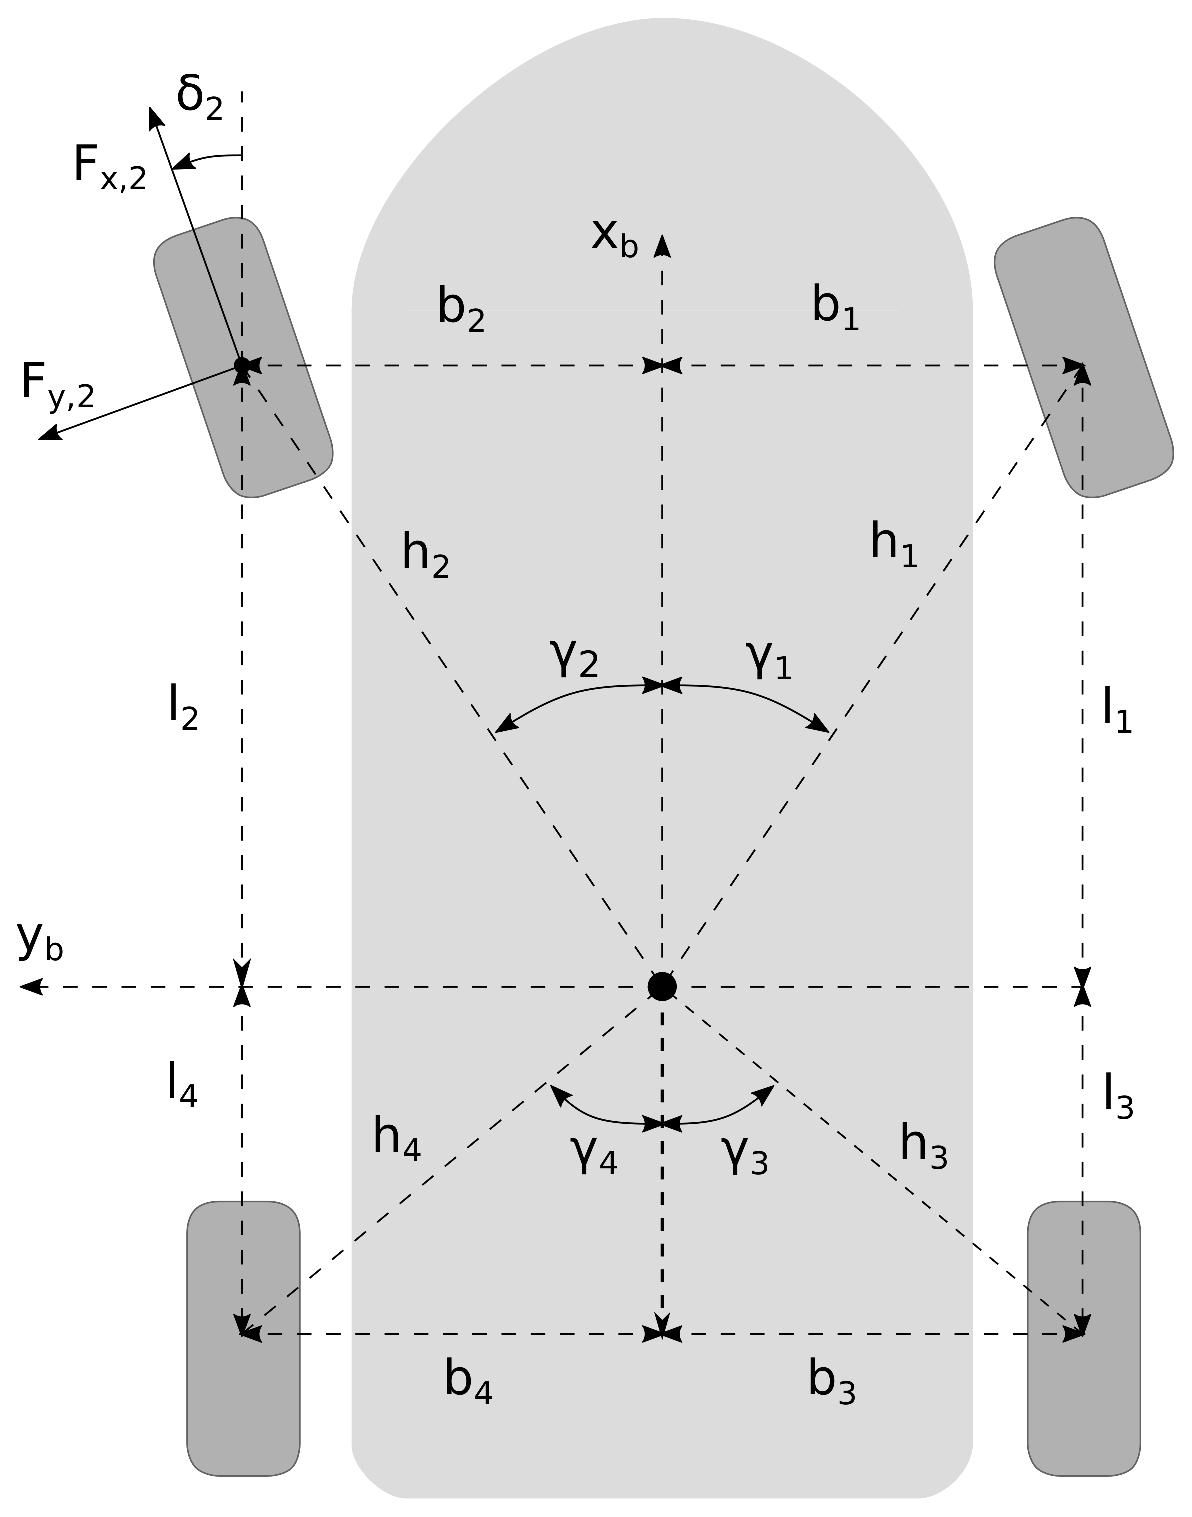
\includegraphics[width=0.5\linewidth]{0_Images/3_Theory/TorqueCalculations.eps}
    \captionof{figure}{Illustrations of variables used for torque calculations.}
    \label{Fig:WheelTorques}
\end{figure}

This estimate is then used in much the same way as for the longitudinal velocity to update our estimate of the yaw rate.

\begin{equation}
    \ddot{\hat{\psi}} = \frac{1}{J}\theta \hat{f}_r^* + k_r(\dot{\psi}-\hat{\dot{\psi}})
\end{equation}

where $J$ is the moment of intertia of the vehicle around CG, and $K_r$ is our faith in the estimate calculated by looking at lateral tyre forces, compared to yaw rate coming out of the IMU. 

\subsubsection{Friction parameter}
Instead of estimating the friction parameter directly, which would have meant one friction coefficient per wheel, we parametrize the lateral force as we have seen earlier

\begin{equation}
    f_y(F_{z,i}, \hat{v_x}, \hat{v_y}, \dot{\hat{\psi}}) =\theta f_y^*(F_{z,i}, \hat{v_x}, \hat{v_y}, \dot{\hat{\psi}}) 
\end{equation}

This is an acceptable simplification, since the formula student track is uniform tarmac without any oil spill or similar. It will only ever change friction coefficient as a result of weather, and then it's reasonable to assume it's going to affect the track evenly since no parts are going to be under a roof. \\ 

The estimate for the simplified friction coefficient is updated using the following observer

\begin{equation}
    \dot{\theta} = K_{\theta}\Lambda (t, \hat{x})\hat{a}_y^*(t,\hat{x})(a_y - \hat{a}_y(t,\hat{x},\theta))
\end{equation}

\subsubsection{Bank and inclination angle}

The final part of the puzzle is estimating the bank and inclination angle so their effect on the lateral and longitudinal forces can be corrected for. We define the tilt of the ground as first an inclination angle $\Theta$ around the vehicles y axis, and then a bank angle $\Phi$ around the now rotated x axis. This leads to the following effect on the dynamics of the car

\begin{align}
    \dot{v}_x & = a_x + \dot{\psi} v_y + g sin(\Theta) \\
    \dot{v}_y & = a_y - \dot{\psi}v_x - g cos(\Theta) sin(\Phi)
\end{align}

We define $\theta_i = sin(\Theta)$ and $\theta_b = cos(\Theta)sin(\Phi)$ and assuming that the bank and inclination angles are small, these are approximately 

\begin{align}
    \theta_i & \approx \Theta \\
    \theta_b & \approx \Phi
\end{align}

We introduce an estimate of $\theta_i$ and $\theta_b$ as

\begin{align}
    \dot{\hat{\theta}}_i & = K_{\theta_i}K_{v_x}(t)(v_{x,rpm} - \hat{v}_x) \\
    \dot{\hat{\theta}}_b & = K_{\theta_b}(a_y-\hat{a}_y(t,\hat{x},\theta)
\end{align}

Where $K_{v_X}$ is, as previously defined, how much faith is put in the longitudinal velocity estimate coming from the wheel RPMs. $K_{\theta_i}$ and $K_{\theta_b}$ are tuning parameters. The observers for $v_y$ and $v_x$ are modified to correct for this bias by adding $g\hat{\theta}_i$ to $\dot{\hat{v}}_x$ and $-g\hat{\theta}_b$ to $\dot{\hat{v}}_y$. 

\subsubsection{When to estimate friction}

Estimating the bank angle and estimating the friction coefficient $\theta$ are conflicting problems, as both are not properly observable at the same time. In \cite{MainStateEst} this is solved by turning of the friction coefficient update when there isn't enough lateral acceleration for it to converge properly, and turning of the bank angle update when estimating updating the friction coefficient. They found that this worked well in most cases, but that when driving in terrain that is both hilly, meaning varying bank angle, and with a low friction coefficient, they needed to estimate both at the same time. \\

To do this they developed a rather complex set of rules for when to turn on and of the two different update laws. We believe this is not needed in our case, since we are driving on flat ground with a slowly varying bank angle and a friction coefficient that never goes down as low as theirs did. They were driving on snow and ice, while the worst condition we will face will be wet tarmac, so as long as we estimate the bank angle regularly, there shouldn't be a need to estimate both bank angle and friction coefficient at the same time. \\

We therefore employ the same switching rule for when to update the friction coefficient as \cite{MainStateEst} and simply turn of the bank angle update when friction coefficient is being updated. To determine when to turn on the friction update we estimate the reference yaw rate found by looking at the wheel torques, and an estimate of $\dot{v}_y$. $\dot{\hat{v}}_y$ found by low pass filtering $a_y - \dot{\psi}\hat{v}_x$. A high value for $\dot{v}_y$ indicates a high level of excitation and that some of the tyres might be in the nonlinear region where it's possible to get information about the friction coefficient. When both these values are high enough we turn on friction update and turn off bank angle update. \\ 

Ref. \cite{MainStateEst} lets the friction coefficient go exponentially to a nominal value of 1 when it isn't being estimated from the sensor data. They argue that dry tarmac will be the normal operating conditions. We chose instead to simply let the coefficient stay at that value when we aren't updating it from the sensor data, seeing how the ground conditions will change rather slowly.

\subsubsection{Final observer}
The full observer has to modes: either it updates the estimate of the bank angle, or it updates the estimate of the friction coefficient. In the first case the full observer is as follows

\begin{align}
    \dot{\hat{v}}_x & = a_x + \dot{\hat{\psi}}\hat{v}_y + g\hat{\theta}_i + K_{v_x}(t)(v_{x,rpm} - \hat{v}_x) \\
    \dot{\hat{v}}_y & = a_y - \dot{\hat{\psi}}\hat{v}_x - g\hat{\theta}_b + K_{v_y}\xi(t,\hat{x})\Lambda(a_y - \theta a_y^{*}) + \frac{\Gamma_2}{\Gamma_1}\zeta(\dot{\psi} - \dot{\hat{\psi}}) \\ 
    \dot{\hat{\theta}}_i & = K_{\theta_i}K_{v_x}(t)(v_{x,rpm} - \hat{v}_x) \\
    \dot{\hat{\theta}}_b & = K_{\theta_b}(a_y-\hat{a}_y(t,\hat{x},\theta)) \\ 
    \ddot{\hat{\psi}} & = \frac{1}{J}\theta \hat{f}_r^* + k_r(t)(\dot{\psi}-\hat{\dot{\psi}})
\end{align}

When updating friction coefficient and not bank angle the observer looks like this

\begin{align}
    \dot{\hat{v}}_x & = a_x + \dot{\psi}\hat{v}_y + g\hat{\theta}_i + K_{v_x}(t)(v_{x,rpm} - \hat{v}_x) \\
    \dot{\hat{v}}_y & = a_y - \dot{\hat{\psi}}\hat{v}_x - g\hat{\theta}_b + K_{v_y}\xi(t,\hat{x})\Lambda(a_y - \theta a_y^{*}) + \frac{\Gamma_2}{\Gamma_1}\zeta(\dot{\psi} - \dot{\hat{\psi}}) \\ 
    \dot{\hat{\theta}}_i & = K_{\theta_i}K_{v_x}(t)(v_{x,rpm} - \hat{v}_x) \\
    \dot{\theta} & = K_{\theta}\Lambda (t, \hat{x})\hat{a}_y^*(t,\hat{x})(a_y - \hat{a}_y(t,\hat{x},\theta)) \\ 
    \ddot{\hat{\psi}} & = \frac{1}{J}\theta \hat{f}_r^* + k_r(t)(\dot{\psi}-\hat{\dot{\psi}})
\end{align}

Uniform Global Asymptotical Stability (UGAS) and Uniform Local Exponential Stability (ULES) of the error of the estimator for $(v_x,v_y,r,\theta)$ was proven in \cite{Automatica08}, while UGAS of the error for the estimator for $(v_x,v_y,\theta, \theta_i, \theta_b)$ was proven in \cite{MainStateEst}. The first of these implies UGAS and UGES of the full observer of $(v_x,v_y, r,\theta, \theta_i, \theta_b)$, as long as the gains on the bank and inclination angle estimates are small enough, and the estimates of $\theta$, $\theta_i$ and $\theta_b$ are limited to a small enough range. This is because UGAS together with ULES implies a certain robustness to small constant biases, which is the effect a wrong estimate of the bank and inclination angles would add to the update laws for $\hat{v}_x$ and $\hat{v}_y$. 

\section{Data association}
\subsection{Choice of method}

\subsection{Design}
The chosen design for the frontend uses ideas from the PDA and compatibility test methods, while simplifying a bit because of the inherent limitiations of the specific problem being solved. The main idea is to compare with the latest map coming out of SLAM, using a compatibility test to associate new measurements with existing landmarks. The measurements that can't be associated to the map are then compared with a list of hypotheses, using the same compatibility test. A hypothesis that gets a new measurement associated to it gets its confidence increased, while the ones that don't get their confidence decreased. The measurements that couldn't get associated to neither the map nor the list of hypotheses gets added to the list of hypotheses. \\

Each measurement coming out of the detection algorithms has a covariance matrix that, in the detection frame (see figure \ref{Fig:DetectionFrame}), is empirically found to be approximately a diagonal matrix where the two diagonal elements are functions of distance. \\

\todo{Fix these placeholder plots and change the text a bit.}

The dependence of the variance on distance is found by placing cones in a known grid and having their position measured as accurately as possibly. Data from the sensors are then recorded and the detection algorithms give their best estimate of the position of the cones. The many measured cones are then binned together with regards to distance, and the errors in bearing and angle is plotted, as can be seen in figures \ref{Fig:CameraRError} and \ref{Fig:CameraPsiError}. The variance of these predictions are then plotted, shown in figures \ref{Fig:CameraRVariance} and \ref{Fig:CameraPsiVariance}. \\ 

The plots clearly show that the variance in distance and angle is a function of distance, which also logically makes sense. A curve is therefore fitted on top of this. A linear fit was found to be best for the variance of the pure geometrically calculated distance estimate, while a second order polynomial was found to give the best fit for the neural net solution. These fits are plotted in figure \ref{Fig:CameraRVarianceFit}. For the variance in the angle however, both the purely geometrically calculated value and the neural net solution got a second order polynomial. These fits are shown in \ref{Fig:CameraPsiVarianceFit}. \\

Similar analysis are done for the two other detection algorithms. This means that when a set of new measurements arrive at the SLAM frontend they consist of a vector of measurements and their covariance matrix in the detection frame.  \\

The covariance matrices in the detection frame, $\Sigma_{detect}$, are then rotated into the body frame using the following formula

\begin{equation}
    \Sigma_{body} = R^T(\alpha)\Sigma_{detect}R(\alpha)
    \label{DetectToBodyRot}
\end{equation}

where 

\begin{equation}
    R(\alpha) = \begin{bmatrix} cos(\alpha) & -sin(\alpha) \\ sin(\alpha) & cos(\alpha)
    \end{bmatrix}
\end{equation} 

and $\alpha$ is the angle between the x-axis of the body frame and the line between CG and the cone in question. \\

\begin{figure}
    \centering
    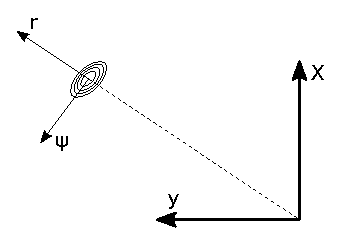
\includegraphics[width=0.5\linewidth]{0_Images/3_Theory/DetectionFrame.eps}
    \caption[The detection frame.]{The detection frame, body frame and height curves of the gaussian noise on the detected cones position.}
    \label{Fig:DetectionFrame}
\end{figure}

\iffalse
\begin{figure}
    \centering
    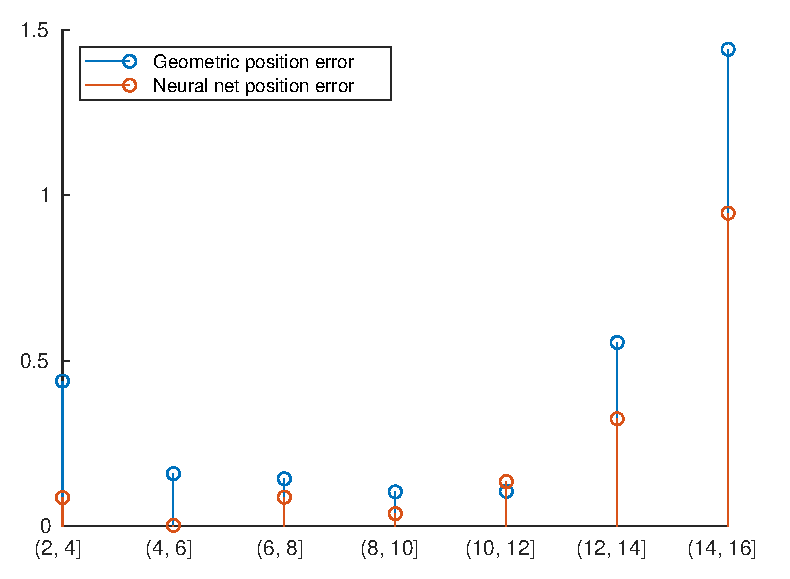
\includegraphics[width=0.5\linewidth]{0_Images/3_Theory/camDetection/rErrorCamera.eps}
    %\captionof{figure}{The error and variance along the r-direction of the camera detection algorithm, using just geometric considerations on %the size of the .}
    \caption[Binned distance error from the camera detection algorithm.]
    {Binned distance error from the camera detection algorithm compared to ground truth. One is using just geometric calculations on the bounding box coming out of the neural net, while the other is a neural net that inputs the bounding box and the geometrically calculated position to give a better position estimate.}
    \label{Fig:CameraRError}
\end{figure}

\begin{figure}
    \centering
    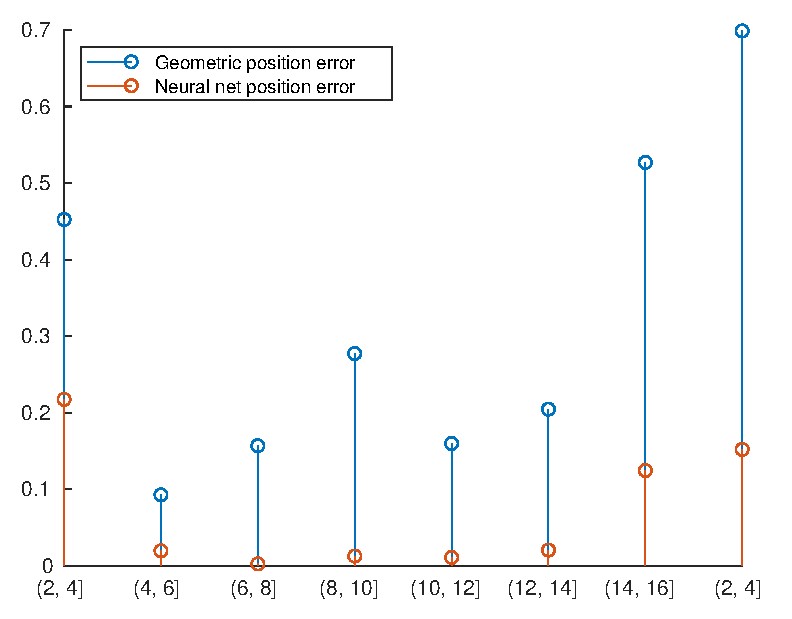
\includegraphics[width=0.5\linewidth]{0_Images/3_Theory/camDetection/psiErrorCamera.eps}
    %\captionof{figure}{The error and variance along the r-direction of the camera detection algorithm, using just geometric considerations on %the size of the .}
    \caption[Binned angle error from the camera detection algorithm.]
    {Binned angle error from the camera detection algorithm compared to ground truth. One is using just geometric calculations on the bounding box coming out of the neural net, while the other is a neural net that inputs the bounding box and the geometrically calculated position to give a better position estimate.}
    \label{Fig:CameraPsiError}
\end{figure}

\begin{figure}
    \centering
    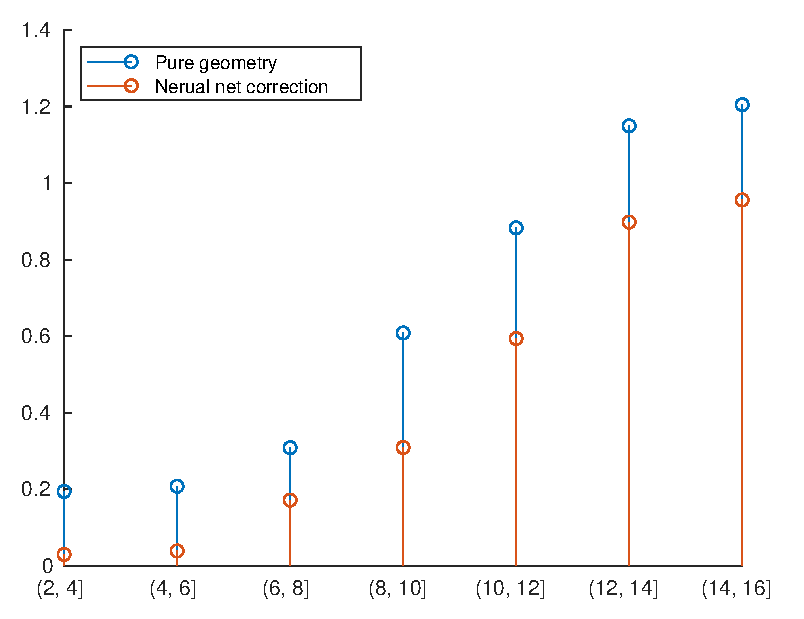
\includegraphics[width=0.5\linewidth]{0_Images/3_Theory/camDetection/rVarCamera.eps}
    %\captionof{figure}{The error and variance along the r-direction of the camera detection algorithm, using just geometric considerations on %the size of the .}
    \caption[Binned distance variance from the camera detection algorithm.]
    {Binned distance variance from the camera detection algorithm compared to ground truth. One is using just geometric calculations on the bounding box coming out of the neural net, while the other is a neural net that inputs the bounding box and the geometrically calculated position to give a better position estimate.}
    \label{Fig:CameraRVariance}
\end{figure}

\begin{figure}
    \centering
    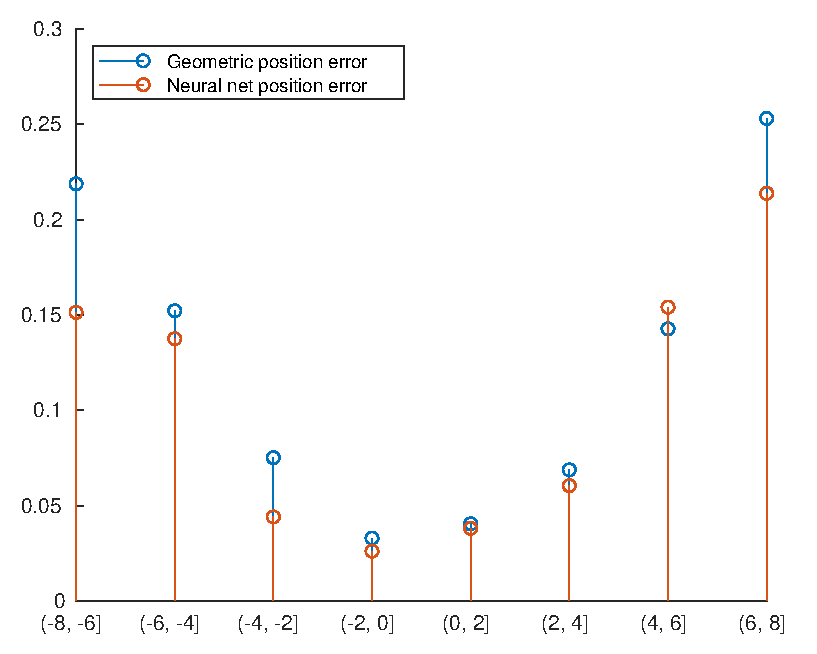
\includegraphics[width=0.5\linewidth]{0_Images/3_Theory/camDetection/psiVarCamera.eps}
    %\captionof{figure}{The error and variance along the r-direction of the camera detection algorithm, using just geometric considerations on %the size of the .}
    \caption[Binned angle variance from the camera detection algorithm.]
    {Binned angle variance from the camera detection algorithm compared to ground truth. One is using just geometric calculations on the bounding box coming out of the neural net, while the other is a neural net that inputs the bounding box and the geometrically calculated position to give a better position estimate.}
    \label{Fig:CameraPsiVariance}
\end{figure}

\begin{figure}
    \centering
    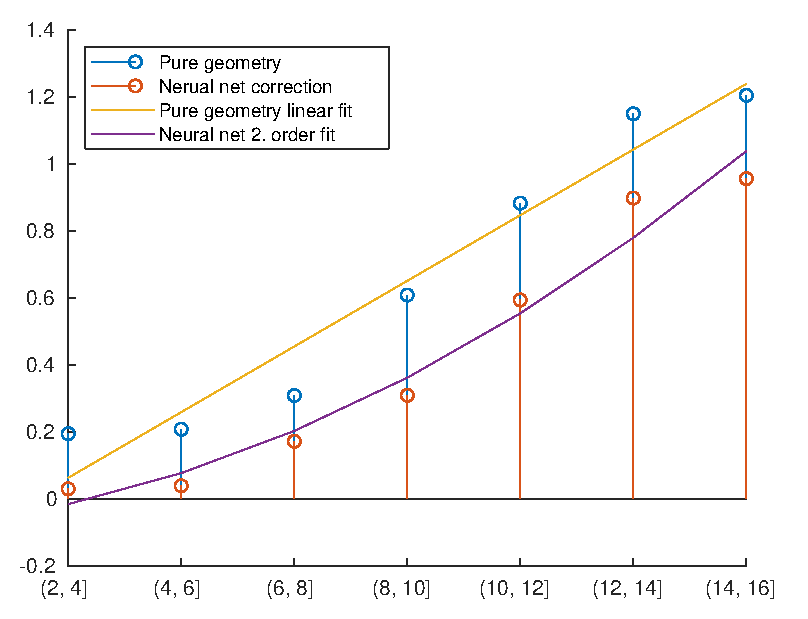
\includegraphics[width=0.5\linewidth]{0_Images/3_Theory/camDetection/CameraRVarianceFit.eps}
    %\captionof{figure}{The error and variance along the r-direction of the camera detection algorithm, using just geometric considerations on %the size of the .}
    \caption[Fitted functions over the r-variance of the camera detection algorithm.]
    {Fitted functions over the r-variance of the camera detection algorithm. The variance of the purely geometrically calculated distance is fitted linearly, while the neural net solution gets a second order polynomial.}
    \label{Fig:CameraRVarianceFit}
\end{figure}

\begin{figure}
    \centering
    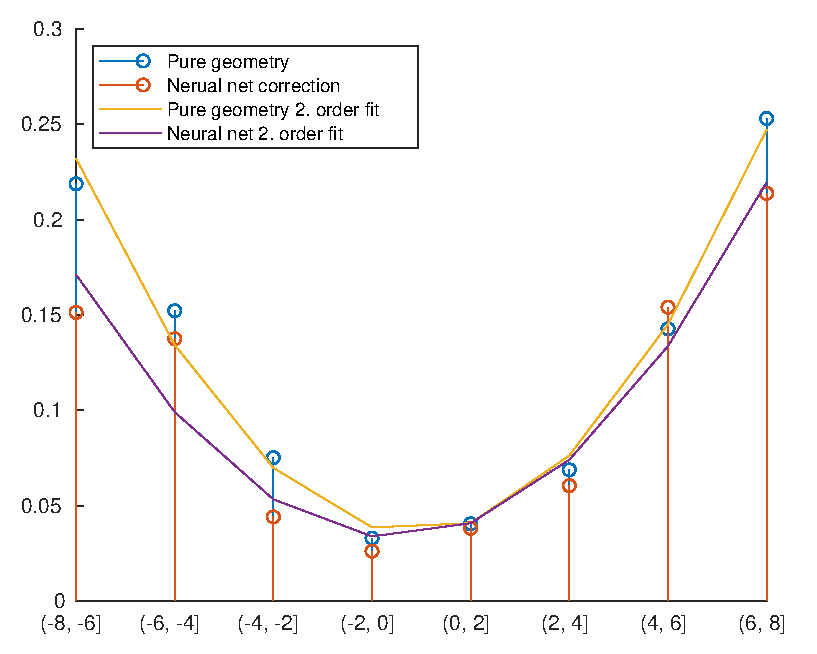
\includegraphics[width=0.5\linewidth]{0_Images/3_Theory/camDetection/CameraPsiVarianceFit.eps}
    %\captionof{figure}{The error and variance along the r-direction of the camera detection algorithm, using just geometric considerations on %the size of the .}
    \caption[Fitted functions over the $\psi$-variance of the camera detection algorithm.]
    {Fitted functions over the $\psi$-variance of the camera detection algorithm. Both the purely geometrically calculated value and the neural net solution got a second order fit.}
    \label{Fig:CameraPsiVarianceFit}
\end{figure}

\fi
\subsection{Comparison with the existing map}

Each detected cone is then transformed into the map frame, using the latest estimate of the cars position coming from the state estimation, as well as the correction on the state estimation that SLAM gives us. Since the last time a detection arrived, the state estimation covariance has been accumulated and is now added to all the landmarks in the map. \\

This accumulation is simply summing of the diagonal covariance matrices of each odometry message, i.e. the covariance in the change of $x$, $y$ and $\psi$. This information arrives as covariances in the body frame, and even though this body frame will rotate and translate with respect to the map frame, it's assumed to never be a very long time between each set of detections arriving. Therefore it's assumed that the step from the last detection can be approximated as a single translation followed by a single rotation. This assumption is used to simplify the process of summing the covariances. \\

Instead of integrating the covariance along the trajectory of the car, the covariance in $x$ and $y$ of the accumulated odometry is simply summed and rotated into the global frame before getting added to the covariance of each landmark in the map. This is of course a simplification, but it avoids having to iterate through the map each time a new odometry message arrives, which is at $\SI{400}{Hz}$, thus leading to a lot of unecessary computation. The team believes this error will be dominated by errors in the covariance estimates, so computation time was chosen over accuracy. \\ 

The yaw covariance is accumulated by summing as well, but increases the covariance of each landmark in a different way. The covariance in yaw of the accumulated step will lead to an increased covariance of each landmark that is approximately aligned with the $\psi$-direction in the detection frame that sits on top of each landmark. The magnitude of this covariance is the accumulated covariance, $\sigma_{\psi}^2$ times the distance, $r$, between the landmark and the car. This leads to a covariance matrix in the detection frame, which is then rotated into the body frame and added to the covariance of the landmark

\begin{equation}
    \Sigma^{new} = \Sigma^{old} + R(\alpha)diag\{0,\sigma^2_{\psi}r\}
\end{equation}

Here $\Sigma^{old}$ is the old covariance of the landmark, $\Sigma^{new}$ is the new and $R(\alpha)$ is the rotation matrix aligning the detection frame with the body frame, defined in equation \ref{DetectToBodyRot}. \\

The closest landmark in the map to each cone is then found, and a compatibility test is done for each detected cone, using the covariance of the detected cone and the covariance of the closest landmark. All positive associations are then sent to SLAM as new measurements to existing landmarks. This information also includes the pose the car was in when it saw the landmarks. \\

Since the track follows some strict rules regarding spacing between landmarks, there will never be  cones too close together. Therefore each landmark has a safety zone around it of about $\SI{1}{meter}$. If a detection is within the safety radius of an already existing landmark, but doesn't pass the compatibility test with it, it gets discarded. This rule might mean discarding the few cones where this is not true, but it also makes the system overall more robust to outliers, so the team believes the trade off is worth it.  All the remaining detections are kept for comparison with the set of hypotheses. \\

\subsection{Comparison with the set of hypotheses}

In the next step, the remaining detections are compared with the list of hyptheses. This is done the same way as for comparing with the map, by increasing the spatial covariance of all hypotheses, and association through a simple compatility test, where the Mahalanobis distance must be below a threshold. One major difference is however that if two detections from the same detection algorithm at the same time step can be associated to the same hypotheses, then both the measurements and the hypotheses are discarded as outliers. This simplification means no care must be taken with overlapping hypotheseses, like what is done in the JPDA. \\

\subsubsection{Positive associations}

A positive association with a hypothesis means that the confidence of this hypothesis is increased, and the measurement is added to the list of measurements of this hypothesis. How much the confidence is increased was initially going to be a function of distance from the car, but the ratio between the number of false and true positives have so far not turned out to be dependent on distance or angle in any meaningfull way. For now the initial confidence is therefore just a function of which detection system the measurement came from. This is because there are fewer false positives from the camera algorithm than from the two LiDAR systems. \\

A positive association also means that the position in the map frame of the hypothesis is updated by a Kalman update step. This is done by first finding the distance between the measured position $z_{k-1}$ and the estimated one, $\hat{x}_{k|k-1}$. Call this distance $\Tilde{x}_k$. To find the optimal weighting between the new measurement and the previous estimate, the so called Kalman gain, $K_k$, is created

\begin{equation}
    K_k = P_{k|k-1}S^{-1}_k
\end{equation}

where 

\begin{equation}
    S_k = R_k + P_{k|k-1}
\end{equation}

is the measurement noise, $R_k$, plus the propagated noise from the previous step, and $P_{k|k-1}$ is the covariance of the landmark. This gain is then used to give a high weight to the measurement when the measurement noise is low and system noise is high, and vice versa. The new estimated position of the landmark is then

\begin{equation}
    \hat{x}_{k|k} = \hat{x}_{k|k-1} + K_k\Tilde{y}_k
\end{equation}

The keen reader might notice that there is no $H_k$ in the above equation. This is because our measurement function is the identity. \\

The new covariance, $P_{k|k}$, of the landmark is then found by  

\begin{equation}
    P_{k|k} = (I-K)(P_{k|k-1} + Q)
\end{equation}

This makes the covariance get smaller if the measurement and previous estimate are close together, and increase if they are far apart. In reality the covariance will always get smaller when a measurement is associated to a hypothesis, because of the compatibility test. \\

\subsubsection{Lack of association}

If a hypothesis isn't associated to when a new set of detections arrive, its confidence is decreased. How much it's decremented by is a function of which detection system this set of detections came from, and whether or not this hypothesis is in the field of view of the detection system. If it is then the confidence is decremented by a number that is a function of distance. \\

This last part has not been implemented yet, just like the initial confidence function, because we yet have no proper estimates of ratio between false positives and true positives as a function of distance. \\

\subsubsection{Belief correction}

When a hypothesis' confidence climbs above a threshold it is accepted as an inlier and all the measurements of it are sent to SLAM as measurements of a new landmark. Similarily when the confidence goes below a threshold it is discarded. A hypothesis is also discarded when it's spatial gets too big. This is because we don't want ambiguity when associating measurements to the hypotheses. \\

The remaining measurements are then initialized as a new hypothesis. It is given an initial confidence that is a function of detection method and distance from the car. This is because when we plot the ratio between true positive and false positives, this ratio goes down as the distance increases. Thus the confidence is initialized at a lower value when the cone is further away. \\


\section{Generating ground truth}

To measure the accuracy of both the SLAM system and the state estimator, as well as for tuning gains in them, good ground truth of both position and velocity is needed. It's also needed by other systems on the car, like for example the detection algorithms. There are several ways of creating this ground truth. One could do measurements by hand, either using a simple yardstick or handheld laser distance measurement. This is however very unreliable, takes a lot of time and effort and is only feasible for position, not velocity. \\ 

Another option is using a system of automatic ranging lasers, but they are expensive and the commercially available ones have low range as they are made for robotics. Such a system could potentially be made from scratch at a much lower cost, but this is very time consuming, and time is one of the scarcest resources at Revolve. \\

Yet another option is visual feature tracking, but this is unreliable, and either time-consuming to make or expensive to buy. The team also doubts whether it works as well for our use, as we want centimeter precision at high speeds and cannot guarantee perfect lightning conditions. \\ 

The team also looked into using the telemetry antenna as ground truth, since it is has $60$ radio antennas in its receiver, and can be configured to output a pretty accurate spherical angle to the car from the antenna. The estimate of time of flight was however not very good, so to get the position in three dimensions another antenna is needed. We are still waiting for this, but if we get it from our sponsor then it looks very promising. As of now though, another way of doing validation is needed. \\

The validation setup the team ended up settling on is a Real-time kinematics global positioning system (RTK-GPS). A base station is set up, sending corrections to the gps system on the car through our telemetry antenna. When the system has enough time to initialize and find a good fix on the position of the base station, and the test area has a good view of the sky without much multipath, then this works very well. \\

It does however mean that testing is a bit more tedious, since the chosen validation method gives constraints on test location and means it takes more time. It also means the ground truth needs some post processing to work well for tuning, removing outliers and parts where the GPS system lost fix on enough satelites.
\chapter{Implementation}
\section{ROS}

For the whole autonomous pipeline, the system used the Robot Operating System (ROS)\cite{ROS}. It claims to be a "meta-operating system", providing a wealth of services that a modern robot system might need, like message-passing between processes, facilitating debugging, visualization, low level device control and packet management. It also includes a standardized framework for working with coordinate system transformations and an abundance of standard and user-made packages for all sorts of operations, libraries and so on. \\

What the team used it for most is package management, providing a unified system for building the whole pipeline, the standardized message passing system and the transformation framework. It also provides an easy interface between the software and many of the cars sensors, like the IMU, converting sensor data into standard message types that are easy to use by the rest of the system. Finally it gave us a nice way of visualizing data, using ROS's RVIZ, and for debugging the communication between the different nodes in the pipeline, using rqt and especially rqt\_graph.
\section{State estimation}

The nonlinear observer used for state estimation was first developed in MATLAB, because it allowed the system to be tested easily on data from last years summer testing period. The IMU data was pretty noisy, since they had not managed to turn on the internal Kalman filter in the VN300, like we have now. This meant that a lowpass filter had to be employed on the yaw rate, as this especially contained a lot of noise. \\

After the observer was tuned and validated on data from last year in MATLAB, it was implemented in c++, using ROS to get the messages in from the sensor and sending out the state estimates. A practical concern was the different output rates of the sensors; the IMU ran at a higher output than the RPM and steering angle sensors. Therefore a "sample and hold" technique was used, always using the latest value of the RPM and steering angle. This was tested on the few ROS-bags that the team had from last year that contained all the right sensor data, and proved not to cause any trouble.  \\

\subsubsection{$v_y$ decay}

When first implementing the observer, it turned out to be very unstable, shooting of into infinity every once in a while. This was fixed by having the estimate of $v_y$ decay towards zero exponentially, by adding a proportional feedback term, with a gain of $0.3$. After this the observer was completely stable.
\section{SLAM}

The SLAM backend was implemented using the GTSAM factor graph frame work\cite{GTSAM}, and more specifically using its iSAM2\cite{iSAM2} library. This allowed us to optimize only the most relevant parts of the graph, thus keeping the run time down. \\

The optimization still uses some time, much more than the frontend. Therefore, in order for the frontend to be able to work without having to wait for the optimization to finish, the frontend and backend is separated into two threads. This makes it possible to both optimize the graph and handle new incoming detections at the same time. \\

The disadvantage is however that the interplay between the two threads need to be controlled. This is done by having the two threads communicate through variables that are locked by mutexes, i.e. only allowing one thread to operate on the variables at a time. The map and odometry information, as well as the list of new measurements and new landmarks being sent from the frontend to the backend are locked by mutexes. This makes sure that no information is lost or corrupted by simultaneous operations on the same variable. \\

Another concern that had to be adresses was how the system could use both the estimated pose of the vehicle in the odometry frame, and the correction from the SLAM backend on the transformation between the odometry frame and the map frame. This was done using the ROS tf framework. It gives access to a lookupTransform function that gives the transformation between any two frames that have all the needed transformation posted on the tf server. Thus the newest estimate of the body frame could be found by querying for the transform between the map and body frames. 
\section{Sensor calibrations}

\subsubsection{Camera}
To find the transformation from the camera frame to the body frame, both the intrinsic parameters and the extrinsic parameters of the camera had to be found. The intrinsic parameters where found using Kalibr\cite{Kalibr1}\cite{Kalibr2}\cite{Kalibr3}, by filming an april grid (figure \ref{Fig:Aprilgrid}) at various angles and distances, and running the whole film through Kalibr. This gives the distortion of the camera with respect to the world, such that using this transformation it was possible to find all the points in the world corresponding to a single pixel in the image frame. \\

The extrinsic parameters, i.e. the transformation from the camera to the CG, where found by simply measuring by hand the translation and rotation from the camera to the body-frame. Attempts where made at using the Kalibr tool for this too, by having it find the transformation between camera and IMU. This worked well on our test trolley, as the test trolley was light enough for us to lift around, giving it the necessary pitch, roll and yaw for the algorithm to work. The car was however not light enough for this, so hand-measurements will have to suffice.

\begin{figure}
    \centering
    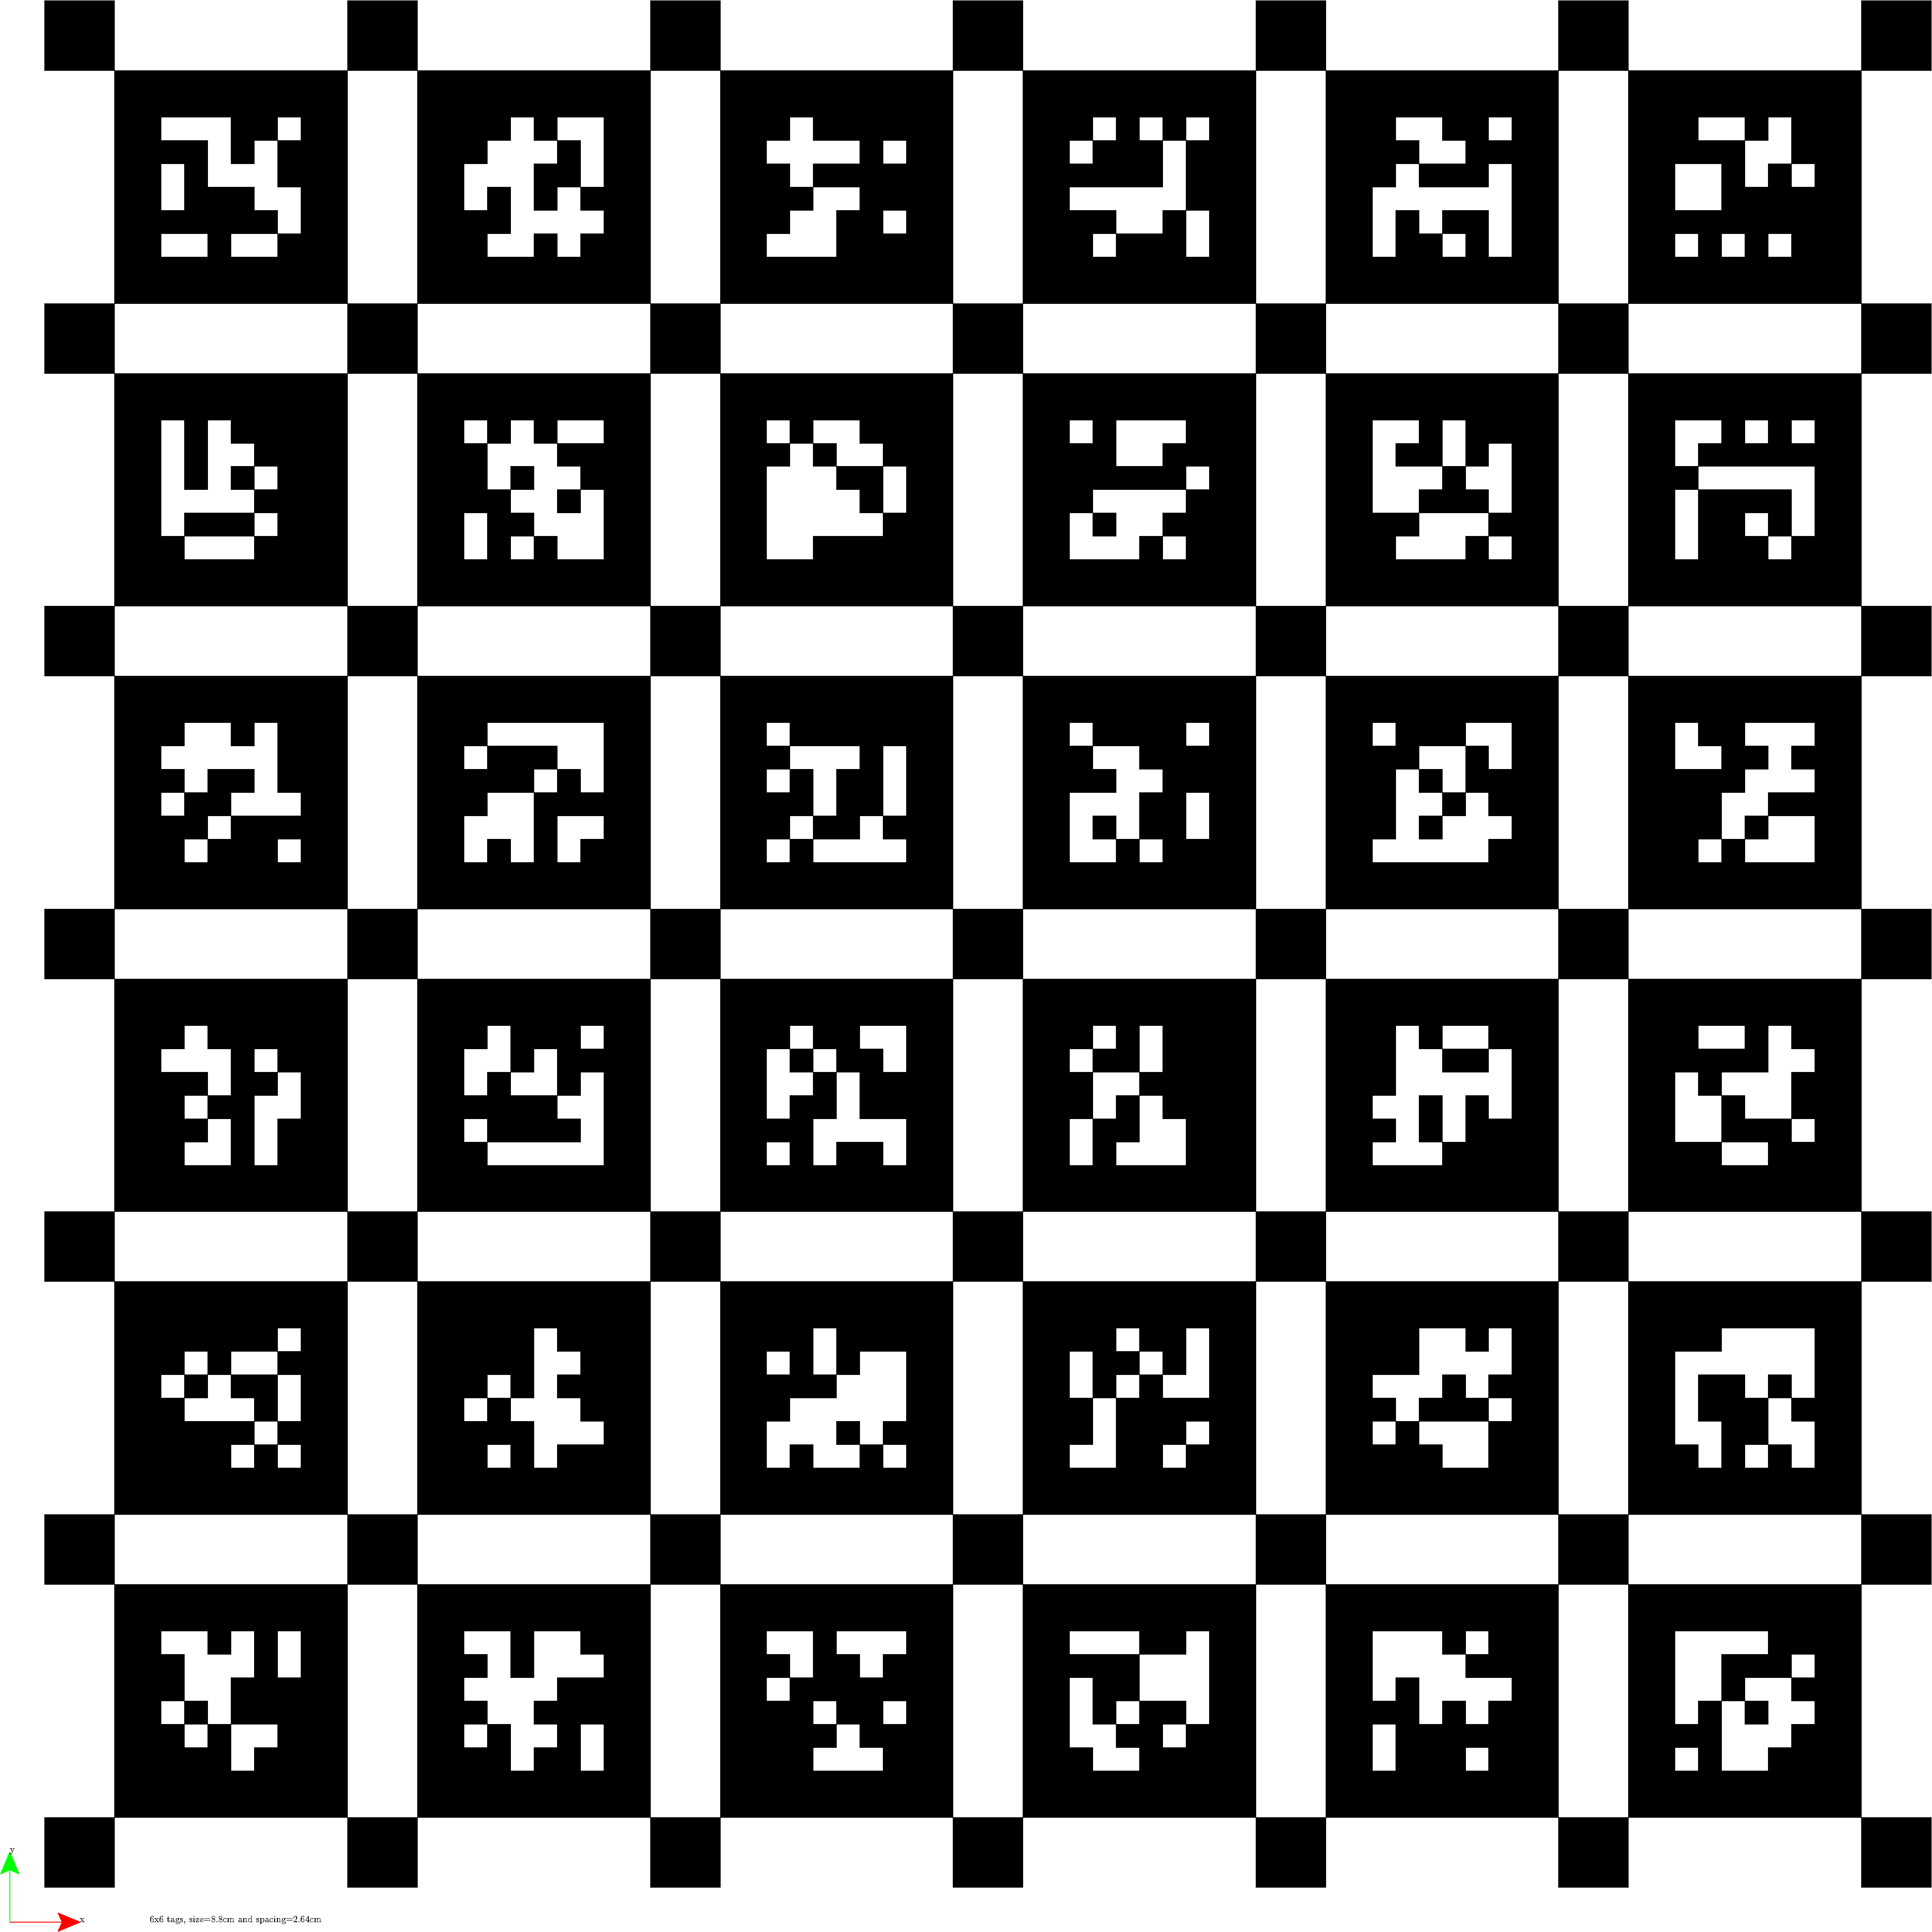
\includegraphics[width=0.5\linewidth]{0_Images/4_Implementation/aprilgrid.pdf}
    \caption[Aprilgrid, the grid used for camera calibration.]
    {Aprilgrid, the grid used for camera calibration.}
    \label{Fig:psiErrorCamera}
\end{figure}

\subsubsection{IMU}

Even though the IMU came with a factory calibration, it was a general one supposed to cover all Vectornav VN300s. So, in order to get a better measurement covariance matrix to send to the built in Kalman filter in the IMU, steps were taken to find the covariance of this specific device. This was done by again using the Kalibr toolbox, but this time for IMU calibration. The device was left alone on a vibration free desk for 8 hours, while recording its output. The output where sent through Kalibr, and the new estimate of the covariance matrix was outputted. This was in turn set to the default value of the VN300. \\

Finding the transformation from the IMU to the body frame was easy as the IMU was placed at what CAD-models in SolidWorks said was the CG. This was done so some of the math in the state estimation algorithm should become easier.

\subsubsection{LiDARS}

To find the transformation from the two LiDARs to the body frame, the transformation from one of them to CG was found by hand measurements. The other one was found by having both LiDARs see a thin stick held stationary. One of the LiDARs where then transformed by trial and error until they both output the same value for the location of the stick. The reaso
\section{Validation setup}
For the validation setup, the team is lucky enough to be allowed access to an industrial area owned by the E. C. Dahls factory here in Trondheim. There we have a pretty flat, open area that resembles the areas used by the competitions we're going to this summer. The area is also free enough from multipaths, thus allowing the use of RTK-GPS for ground truth generation of position and velocity. \\

The location of the cones will then either be measured by hand using a yard stick, or by hand held laser measurement device if this turns out to work well. The team has some ideas for how to use the hand held laser to find the x and y easily, but we won't know if this works until the test period has begun. 

At the test area we will replicate the different track setups that are specified in the formula student rule set. This setup will hopefully be close enough to the real deal to allow us to work about any problems that arise. Unfortunately the car is not ready for testing before the deadline of this project thesis. All the results are therefore from recorded data from last year in the case of the state estimator, and from simulated data in the case of the SLAM system. \\






\chapter{Results}
\section{State estimation}

Graphs with true and estimated states. Graphs with the error in state estimation, both rotation and location, as a function of time? Also have the error/s as a function of speed and rotational speed, and maybe also as a function of acceleration? Drop this last part, don't see the use. \\ 

To validate the algorithm, three sets of data that had good RTK-GPS information was found. Two sets are from the actual dynamic event called "Endurance" during the two competition Formula Student Spain (FSS) and Formula Student Germany (FSG). These two datasets are called "FSS Endurance" and "FSG Endurance", respectively. The last data set is from a test track at FSG that the team had access to in the days before the competition started, called "FSG Test Track 1". \\

The RTK-GPS data were all corrupted by sporadic outliers, so a preprocessing step to remove them was done. A preprocessing step of the yaw angle data was also needed, since the internal kalman filter of the RTK-GPS restricted the yaw to the interval $SI{[-\pi,pi]}{radians}$. \\

The data sets all had varying degrees of quality of the ground truth. They did however all suffer more or less the same from one rather large flaw; last years team had not managed to turn on the internal kalman filtering of the IMU data. This has been corrected now, but this means that the results shown below are different than what is going to be seen when the test period begins. \\

\subsubsection{Ground truth quality}

The first data set, "FSS Endurance", had no GPS position data that was usable, but the longitudinal velocity and yaw rate where both good, as well as the yaw angle. The lateral velocity is usable, but definitely not perfect. It can't be considering how large the sideslip angles can get, regularily going up to values of $10-15 degrees$, which after discussing with the drivers at the event and the vehicle dynamics group seem unreasonably high. The car is not built to sideslip that much at those velocities, nor are the drivers instructed to drive so recklessly, especially not during the endurance event where saving energy is key. \\

The results of the state estimator compared to ground truth for longitudinal  and lateral velocity, yaw rate and yaw angle on the "FSS Endurance" is seen in figures \ref{Fig:VxFSSEndurance}, \ref{Fig:VyFSSEndurance}, \ref{Fig:RFSSEndurance}, \ref{Fig:YawFSSEndurance}, respectively. The integrated position without ground truth is shown in \ref{Fig:PosFSSEndurance}. \\

The second data set, "FSG Endurance", had good position data, as well as good longitudinal velocity and yaw angle. The lateral velocity and yaw rate where however not good enough to use for comparison. The results compared with ground truth for this data set is shown in \ref{Fig:PosFSGEndurance}, \ref{Fig:YawFSGEndurance} and \ref{Fig:VxFSGEndurance}. \\

The last data set, "FSG Test Track 1", like data set 1, had no usable position data, but the longitudinal velocity, yaw rate and yaw angle were all good. The lateral velocity is okay, at least we don't have any reason to not trust it, as it was a really short track with a lot of turning, and the data seems to fit with the way they would have driven it and the way the car was expected to behave. \\

The results of the state estimator compared to ground truth for longitudinal  and lateral velocity, yaw rate and yaw angle on the "FSG Test Track 1" is seen in figures \ref{Fig:VxFSGTestTrack}, \ref{Fig:VyFSGTestTrack}, \ref{Fig:RFSGTestTrack}, \ref{Fig:YawFSGTestTrack}, respectively. The integrated position without ground truth is shown in \ref{Fig:PosFSGTestTrack}. \\



\begin{figure}
    \centering
    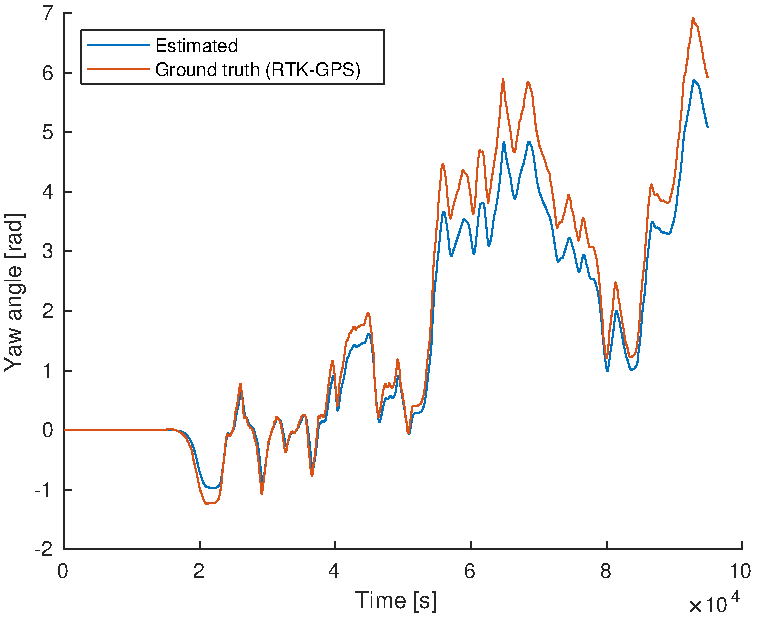
\includegraphics[width=0.8\linewidth]{0_Images/6_Results/yawFSSEndurance.pdf}
    \caption[Yaw angle while driving FSS Endurance.]
    {Yaw angle while driving FSS Endurance. Estimated compared with data from the RTK-GPS.}
    \label{Fig:YawFSSEndurance}
\end{figure}

\begin{figure}
    \centering
    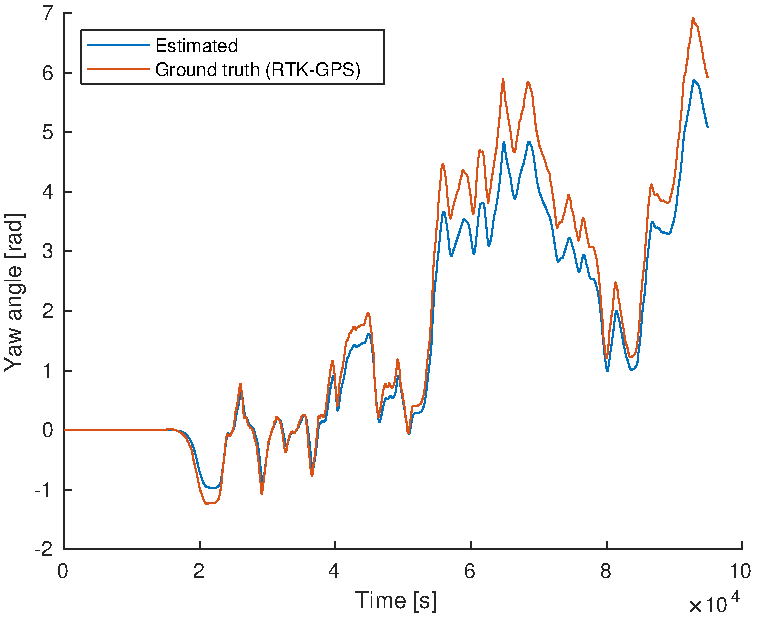
\includegraphics[width=0.8\linewidth]{0_Images/6_Results/yawFSSEndurance.pdf}
    \caption[Yaw angle while driving FSS Endurance.]
    {Yaw angle while driving FSS Endurance. Estimated compared with data from the RTK-GPS.}
    \label{Fig:YawFSSEndurance}
\end{figure}

\begin{figure}
    \centering
    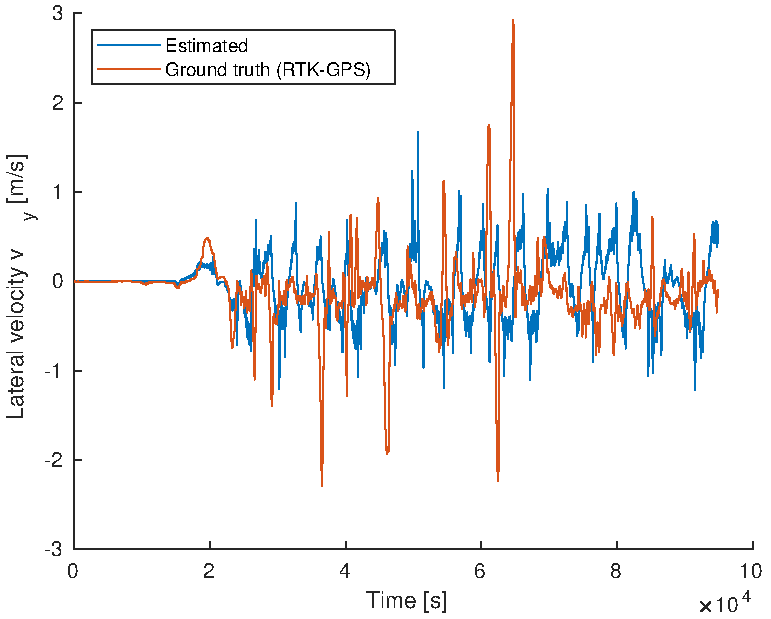
\includegraphics[width=0.8\linewidth]{0_Images/6_Results/vyFSSEndurance.pdf}
    \caption[Lateral velocity while driving FSS Endurance.]
    {Lateral velocity while driving FSS Endurance. Estimated compared with data from the RTK-GPS.}
    \label{Fig:VyFSSEndurance}
\end{figure}

\begin{figure}
    \centering
    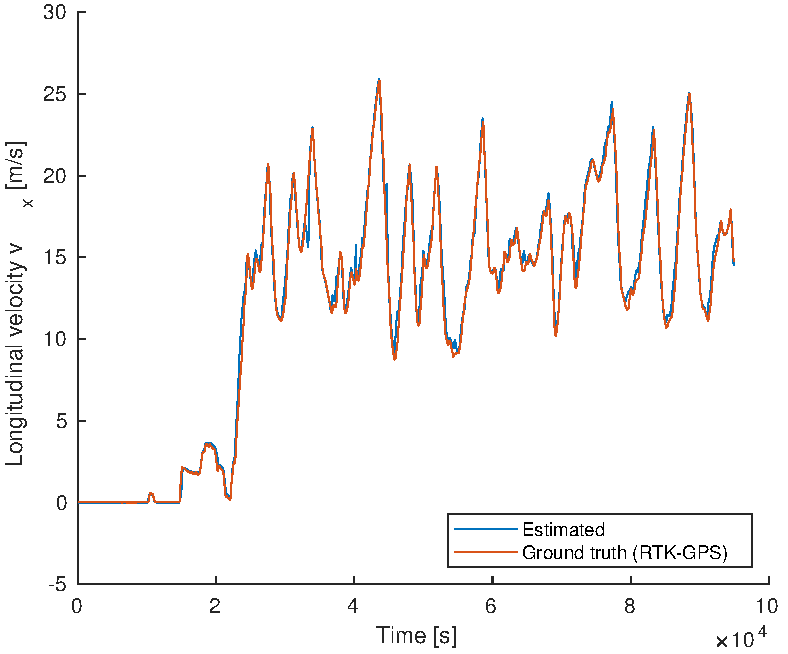
\includegraphics[width=0.8\linewidth]{0_Images/6_Results/vxFSSEndurance.pdf}
    \caption[Longitudinal velocity while driving FSS Endurance.]
    {Longitudinal velocity  while driving FSS Endurance. Estimated compared with data from the RTK-GPS.}
    \label{Fig:VxFSSEndurance}
\end{figure}

\begin{figure}
    \centering
    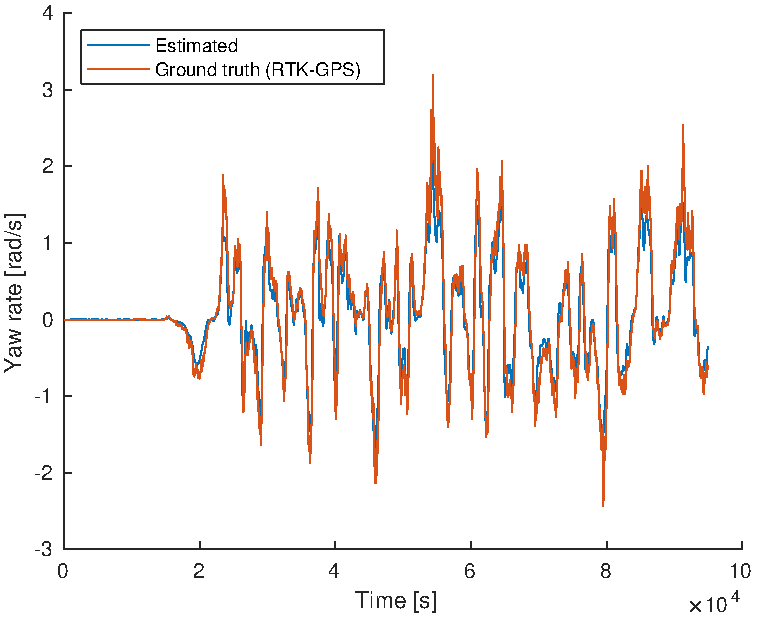
\includegraphics[width=0.8\linewidth]{0_Images/6_Results/rFSSEndurance.pdf}
    \caption[Yaw rate while driving FSS Endurance.]
    {Yaw rate  while driving FSS Endurance. Estimated compared with data from the RTK-GPS.}
    \label{Fig:RFSSEndurance}
\end{figure}

\begin{figure}
    \centering
    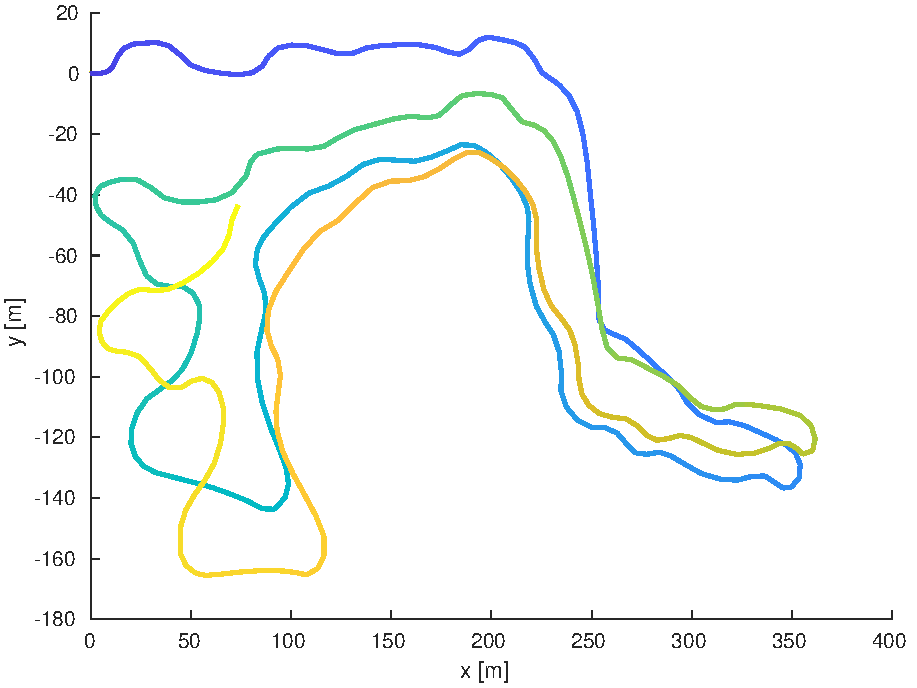
\includegraphics[width=0.8\linewidth]{0_Images/6_Results/positionFSSEndurance.pdf}
    \caption[Position while driving FSS Endurance.]
    {Position while driving FSS Endurance.}
    \label{Fig:PosFSSEndurance}
\end{figure}

\begin{figure}
    \centering
    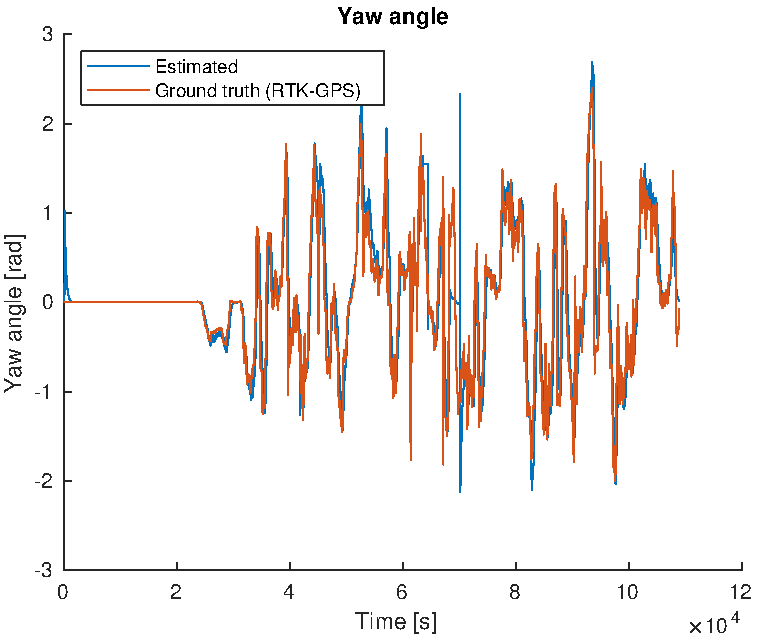
\includegraphics[width=0.8\linewidth]{0_Images/6_Results/yawFSGEndurance.pdf}
    \caption[Yaw angle while driving FSG Endurance.]
    {Yaw angle while driving FSG Endurance. Estimated compared with data from the RTK-GPS.}
    \label{Fig:YawFSGEndurance}
\end{figure}

\begin{figure}
    \centering
    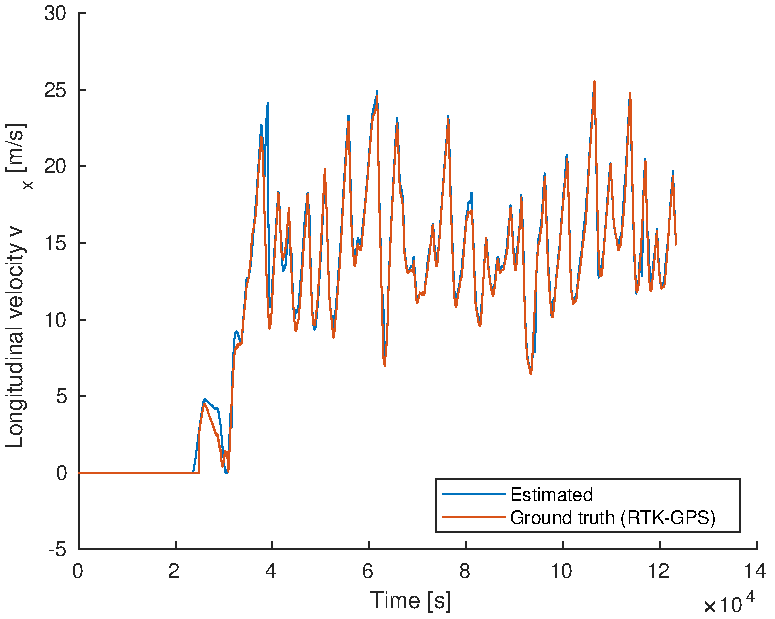
\includegraphics[width=0.8\linewidth]{0_Images/6_Results/vxFSGEndurance.pdf}
    \caption[Longitudinal velocity while driving FSG Endurance.]
    {Longitudinal while driving  during FSG Endurance. Estimated compared with data from the RTK-GPS.}
    \label{Fig:VxFSGEndurance}
\end{figure}

\begin{figure}
    \centering
    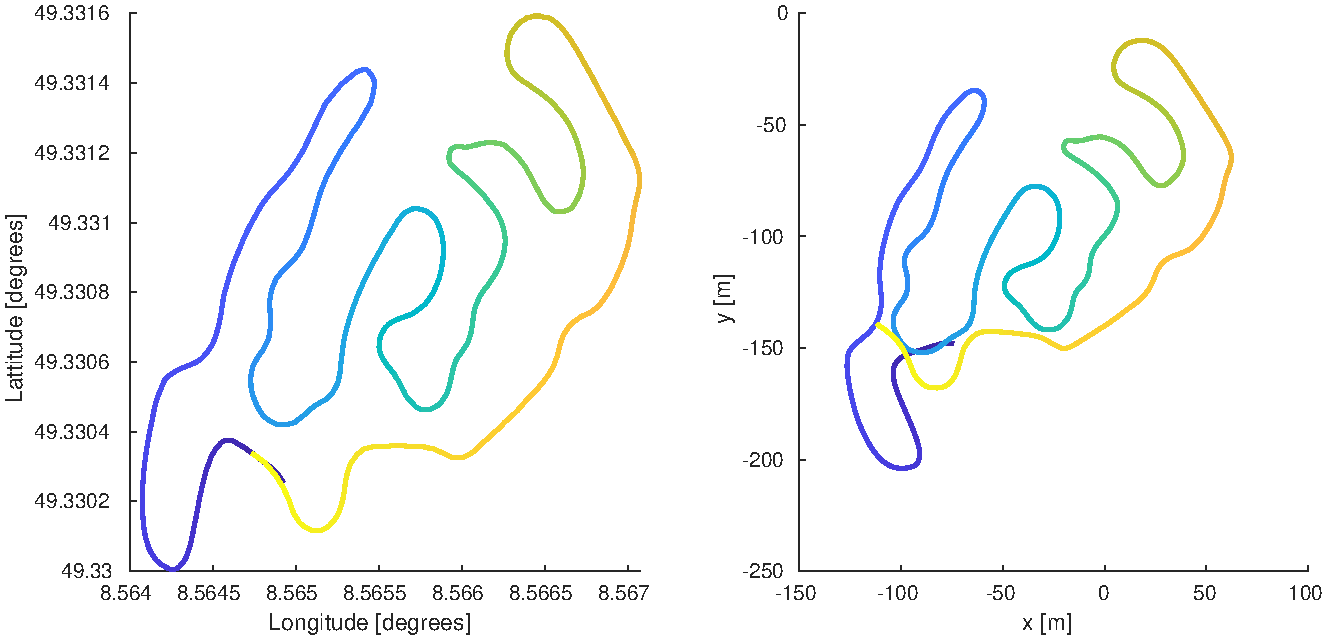
\includegraphics[width=0.8\linewidth]{0_Images/6_Results/positionFSGEndurance.pdf}
    \caption[Position while driving FSG Endurance.]
    {Position while driving FSG Endurance. Estimated compared with data from the RTK-GPS.}
    \label{Fig:PosFSGEndurance}
\end{figure}

\begin{figure}
    \centering
    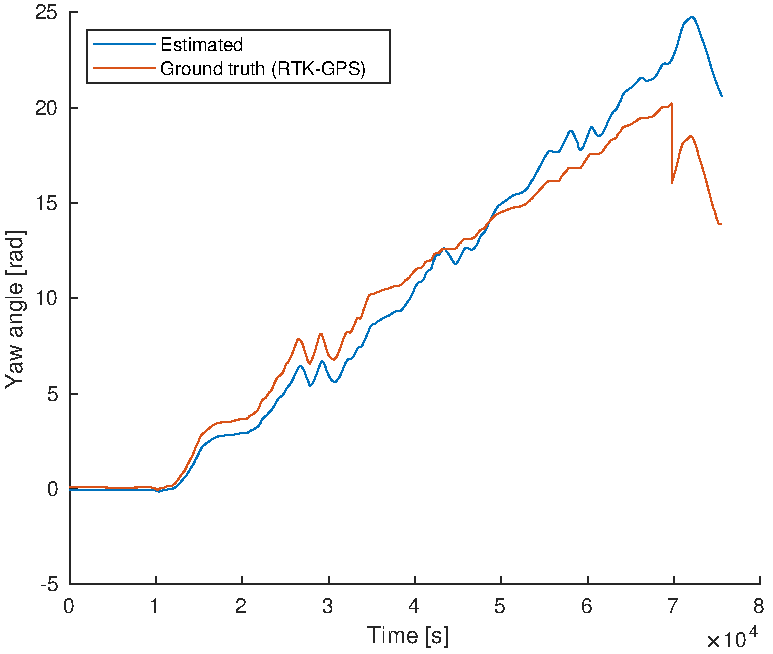
\includegraphics[width=0.8\linewidth]{0_Images/6_Results/yawFSGTestTrack.pdf}
    \caption[Yaw angle while driving FSG Test Track 1.]
    {Yaw angle while driving FSG Test Track 1. Estimated compared with data from the RTK-GPS.}
    \label{Fig:YawFSGTestTrack}
\end{figure}

\begin{figure}
    \centering
    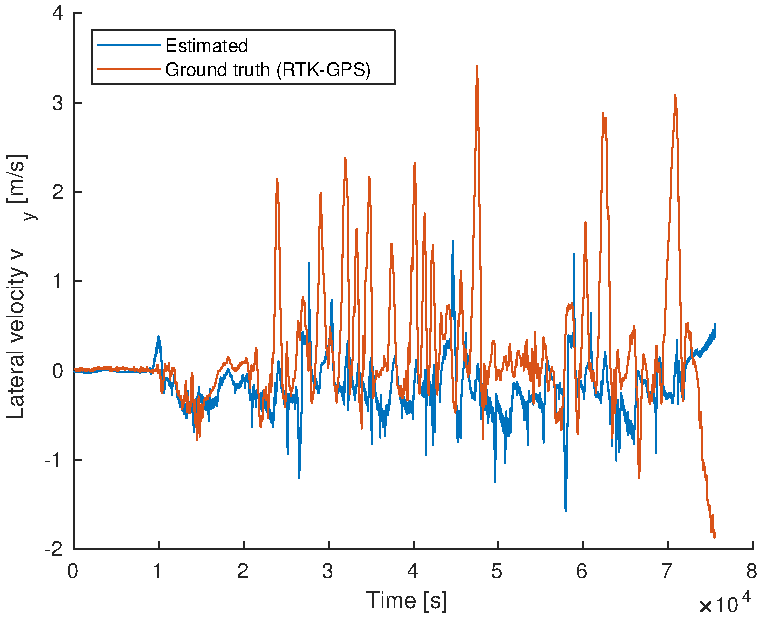
\includegraphics[width=0.8\linewidth]{0_Images/6_Results/vyFSGTestTrack.pdf}
    \caption[Lateral velocity while driving FSG Test Track 1.]
    {Lateral velocity  while driving FSG Test Track 1. Estimated compared with data from the RTK-GPS.}
    \label{Fig:VyFSGTestTrack}
\end{figure}

\begin{figure}
    \centering
    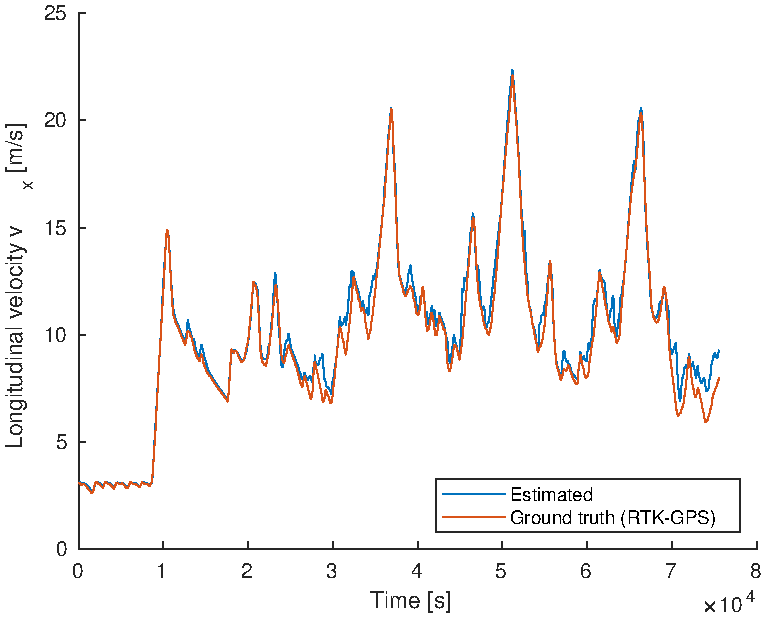
\includegraphics[width=0.8\linewidth]{0_Images/6_Results/vxFSGTestTrack.pdf}
    \caption[Longitudinal velocity while driving FSG Test Track 1.]
    {Longitudinal velocity while driving FSG Test Track 1. Estimated compared with data from the RTK-GPS.}
    \label{Fig:VxFSGTestTrack}
\end{figure}

\begin{figure}
    \centering
    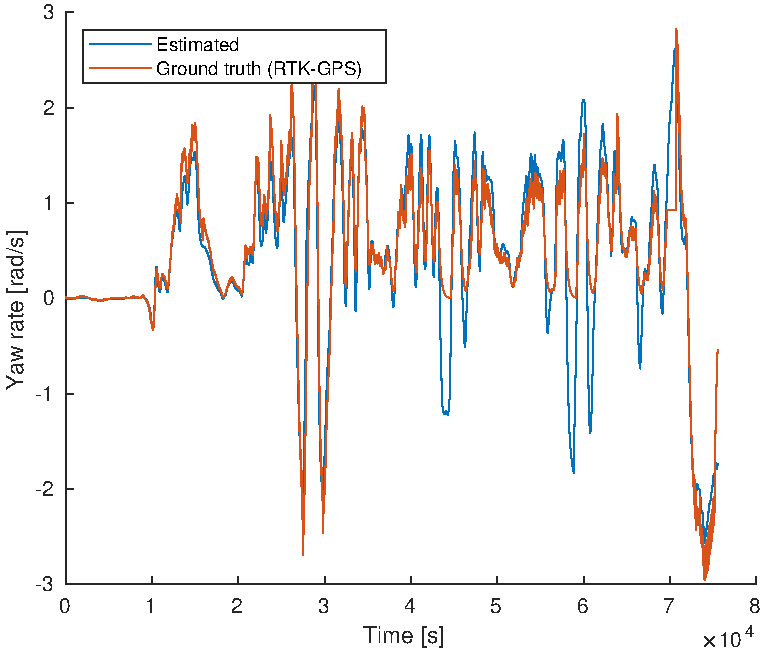
\includegraphics[width=0.8\linewidth]{0_Images/6_Results/rFSGTestTrack.pdf}
    \caption[Yaw rate while driving FSG Test Track 1.]
    {Yaw rate while driving FSG Test Track 1. Estimated compared with data from the RTK-GPS.}
    \label{Fig:RFSGTestTrack}
\end{figure}

\begin{figure}
    \centering
    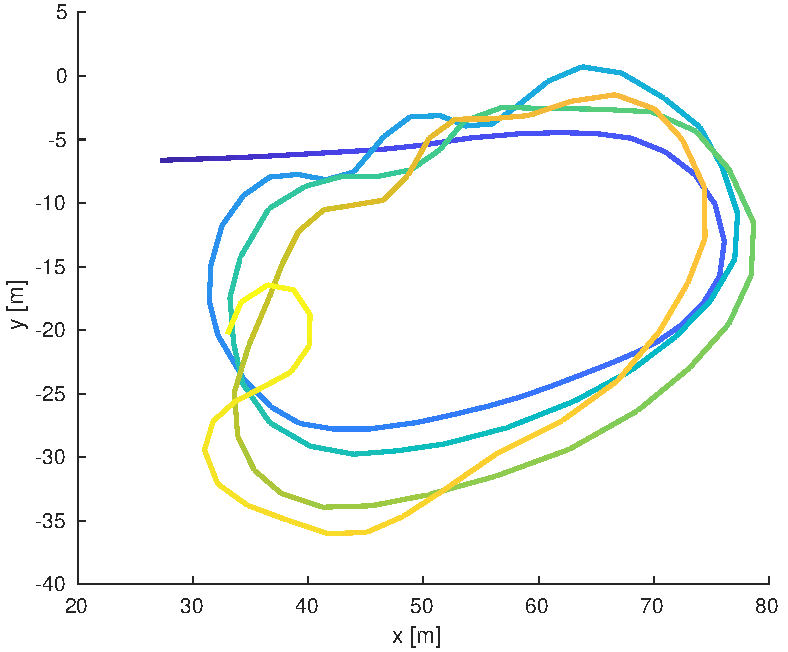
\includegraphics[width=0.8\linewidth]{0_Images/6_Results/positionFSGTestTrack.pdf}
    \caption[Position while driving FSG Test Track 1.]
    {Position while driving FSG Test Track 1.}
    \label{Fig:PosFSGTestTrack}
\end{figure}

\section{SLAM}

We don't really have too many results to show in regards to the SLAM, as we don't get to test it on anything else than simulator until the car is ready, which is going to be some time after this project thesis is delivered. \\

Possible things I can plot:
\begin{itemize}
    \item runtime? Maybe both frontend and backend in one plot?
    \item Map error compared with ground truth as a function of detection noise? Much work \:(
    \item Size of hypotheses-list over time?
\end{itemize}

When simulating with false positives generated with a random gaussian position, the frontend doesn't let any false positives through. This is of course not the best metric for performance, since detection systems don't really send false positives with completely random position. The ones they send are usually because of objects around the track, like walls, and will be spatially correlated. This means that the frontend will have to deal with false positives that cluster around partiular areas. Detection data from last year shows that the false positives that get detected usually jump around a lot, so hopefully the frontend will spawn many new hypotheses that loose confidence, instead of associating to the same false positive and evntually sending it through to the backend. This is not possible to test at the moment unfortunately, since the data from last year isn't compatible with the current system. \\

\begin{figure}
    \centering
    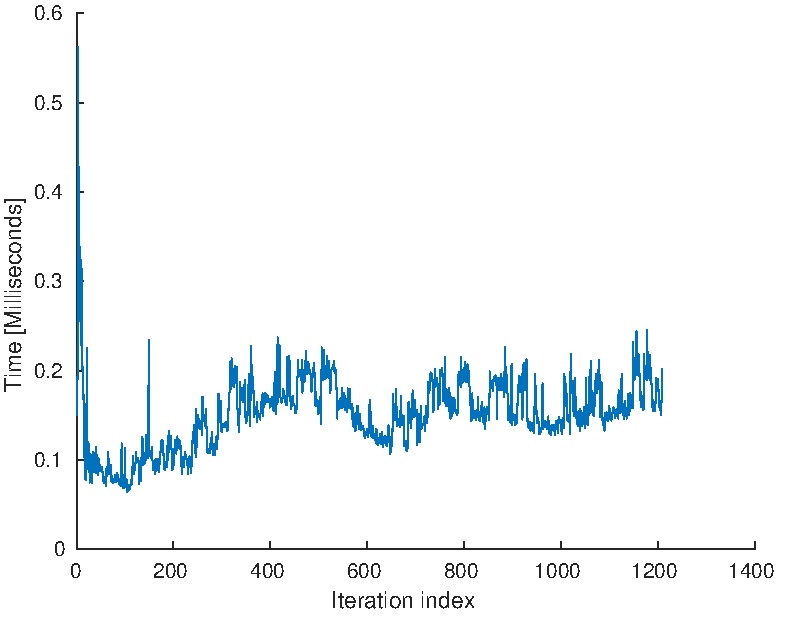
\includegraphics[width=0.8\linewidth]{0_Images/6_Results/FrontendTiming.pdf}
    \caption[Runtime of the SLAM frontend.]
    {Runtime of the SLAM frontend over time, when simulating with gaussian noise on detection and odometry. The timing is from when the set of detection arrives from one of the detection systems to when it is done processing. Simulated using the track from FSG's Autocross event 2018.}
    \label{Fig:FrontendTiming}
\end{figure}

\begin{figure}
    \centering
    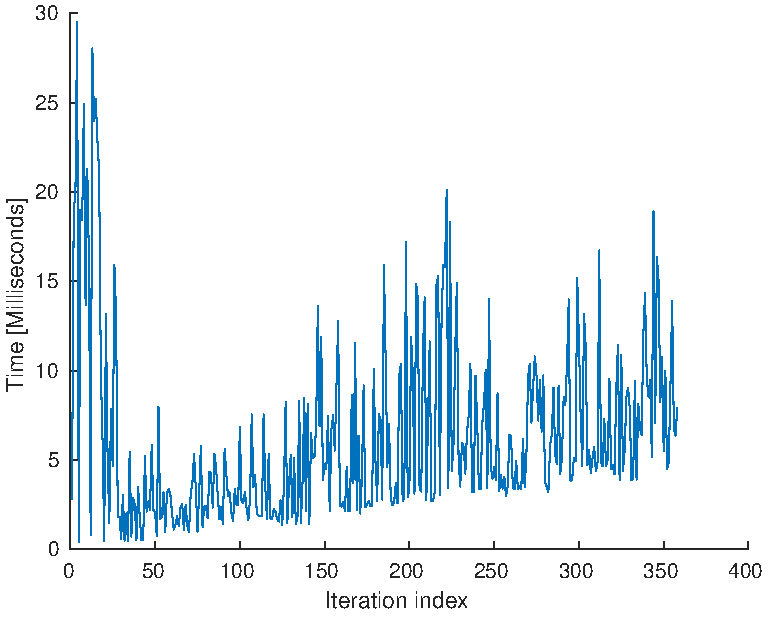
\includegraphics[width=0.8\linewidth]{0_Images/6_Results/BackendTiming.pdf}
    \caption[Runtime of the SLAM backend.]
    {Runtime of the SLAM backend over time, for one complete update. One update means adding all the new information to the graph, optimizing the graph and then sending out the map and pose correction. Simulated using the track from FSG's Autocross event 2018.}
    \label{Fig:BackendTiming}
\end{figure}

\begin{figure}
    \centering
    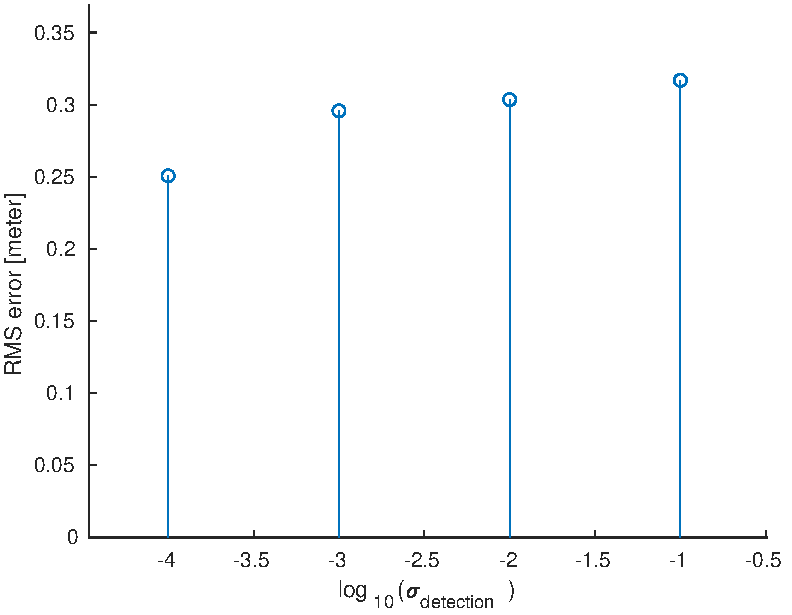
\includegraphics[width=0.8\linewidth]{0_Images/6_Results/SLAMERMS.pdf}
    \caption[SLAM RMS error as a function of logarithm of the standard deviation on the noise added to the detections.]
    {SLAM RMS error as a function of logarithm of the standard deviation on the noise added to the detections. Simulated on one full round around the FSG autocross event 2018. Simulated ten times for each value of the standard deviation and the mean of the rms errors was taken.}
    \label{Fig:SLAMERMS}
\end{figure}
\chapter{Conclusion}
\section{Low average error}

Hopefully we have a low enough average error in state estimation, localization and mapping to be able to say wow what a low average error we have.
\section{Robustness}

Looking at the spikes of the errors, we can hopefully say that they are low, and that the system as a whole is robust to local errors because of SLAM and yada yada.

\section{We won't know if it works well until we have won the competition.}
\chapter{Future work}
Due to the nature of the competition, this whole year has been colored by time pressure. There are therefore several places where there is room for improvement, as the team was constantly forced to take desicions on what would most benefit the team to do. Below are suggestions for future work that the author feels might benefit the team and should be investigated further.

\subsubsection{State estimation}
To improve the state estimation, the team should try to get a sponsorship deal with a company making high quality optical sensors. Adding this speed over ground estimate would improve the state estimation a lot, since these are extremely precise, at least when the ground is dry. However, since their performance degrade a lot when the road is wet, this would also need to be coupled with a system that estimates the wetness of the ground. The speed over ground sensor should then not be trusted, so a nice switching rule would also need to be implemented. \\

If a sponsorship deal cannot be made, it's of the authors opinion that such a sensor does not give enough improvements to warrant the price. The team should keep an ear to the ground and get one if they ever overcome the obstacle of wet tarmac, as it then could be used directly as the only source of state estimation, and one could use the processing power elsewhere.

\subsubsection{Roll estimation}
Since the car rolls an non negible amount when cornering, a good next step would be to estimate the roll angle. This could then be used in the detection algorithms to compensate for roll in the position estimate, or by making the whole factor graph work in 6DOF instead of 3DOF. This would however mean more processing power would be needed for the whole optimization, so there is definitely a trade off.

\subsubsection{GPU acceleration of optimization algorithms}
Since processing power and processing time needs to be as small as possible to give room for the other systems on the car and facilitate real time processing so the car can drive fast, GPU acceleration of the optimization algorithms used to optimize the factor graph is a good next step for the team. It is not clear to the author how large of a task this is, so investigations need to be made prior to commiting to this.\\ 

A good first step is to identify areas of the code that are used a lot and do the same operation many times over. Then try implementing it in CUDA, and time it to see if the cost of moving variables to the GPU memory outweights the lowered processing time used on the calculations. 

\subsubsection{Use planned path when setting initial confidence}
Because of the nature of the track we're trying to map, knowledge about some cones also gives a higher prior on where other cones are located. This means that a natural next step for the team would be to use the possible path coming out of the path planning node to set a higher confidence on measured cones if the cone is close to half a trackwidth away from the planned path. \\

This is of course not without cost. The team should test if this is feasible in terms of computational time, especially when running the full pipeline. It should also be verified that this does not cause more instability in the path planning. A feedback loop of this type could mean the system more easily plans a path that brings the car out of the track. However, this does have the possibility of improving the planning range by a lot, which in the authors opinion makes it worth investigating.

\newpage
%\addcontentsline{toc}{section}{References} %uncomment if you want the references included in the table of content
\bibliographystyle{plain}
\bibliography{ref.bib}


\end{document}
